\chapter{统计推断的理解运用}

\section{多元回归}

\subsection{数据生成过程}

\textbf{基本概念}  

科学研究的核心在于揭示数据背后的生成机制。可知论认为宇宙的运行遵循特定规律,这些规律决定了观测数据的生成方式。这种支配数据生成的潜在机制被称为\textbf{数据生成过程(Data Generating Process, DGP)},它是进行统计推断和因果分析的基础。

DGP是一组隐藏在数据背后的规律性法则。虽然我们无法直接观测这些法则,但能通过其产生的数据进行反向推导。例如,当物体自由下落时,我们观察到的是下落现象,而支配这一现象的本质规律——重力,正是该过程的DGP组成部分。

\textbf{自然科学中的应用} 

以牛顿万有引力定律为例,其数学表达式为:  
\begin{equation}
    F = G \frac{m_1 m_2}{r^2}
\end{equation}  
其中$G$为万有引力常数,$m_1$、$m_2$为物体质量,$r$为距离。这个方程揭示了天体运动背后的DGP。牛顿正是通过观测行星轨迹数据,成功推导出这一规律,从而揭示了引力作用的本质。

\textbf{社会科学中的应用}  

相较于自然科学,社会科学的DGP通常具有更强的复杂性与不确定性。但只要承认观测数据存在某种程度的规律性,就必然存在对应的DGP。理解DGP的关键在于把握两个维度:  
\begin{enumerate}
    \item \textbf{已知规律}:利用既有知识指导数据分析
    \item \textbf{未知规律}:通过研究揭示新的规律性
\end{enumerate}  

以发色与收入的关系研究为例,掌握DGP有助于控制混杂因素(如教育水平、职业选择等),从而获得更精准的因果效应估计。研究者可通过设定特定DGP生成模拟数据,这种"上帝视角"的数据构建方式能完整掌控生成机制,为方法验证提供理想实验环境。例如在收入研究中,可设定:

\begin{itemize}
    \item 收入服从对数正态分布
    \item 棕发群体收入提升10\%
    \item 20\%人口天生棕发
    \item 大学学历带来20\%收入溢价(30\%人口具有学历)
    \item 40\%非棕发低学历者选择染棕发
\end{itemize}  

在这种设定下,简单比较全样本会得出棕发者收入仅高1\%的错误结论。只有通过DGP分析,控制学历等混杂变量,才能在大学生子样本中得到13\%的准确效应估计。

DGP为数据分析提供了系统性框架:  
\begin{enumerate}
    \item \textbf{变异分析}:聚焦目标变量的特征差异(如大学生群体的发色收入差异)
    \item \textbf{因果识别}:确保观测到的变异真实反映目标效应,而非其他因素的干扰(如排除非大学生染发行为的影响)
\end{enumerate}  

掌握DGP的本质规律,既能利用已知规律指导分析,又能揭示未知规律,这是实现精准统计推断、回归分析和因果推断的关键基础。

\subsection{理解线性回归}

继续上文,线性回归模型可以表示为:
\begin{equation}
	INC = \beta_0 + \beta_1 EDU + \beta_2 IQ + \varepsilon
\end{equation}
其中,$Y$是因变量,$EDU$和$IQ$是自变量(解释变量),$\varepsilon$是扰动项。

我们可以绘制一个韦恩图,将各个变量的可能方差变异关系绘制为集合,并寻找哪些部分之间形成了相互影响,图\ref{fig:venn}是一个示例图:

\begin{figure}[ht]
	\centering
	\fbox{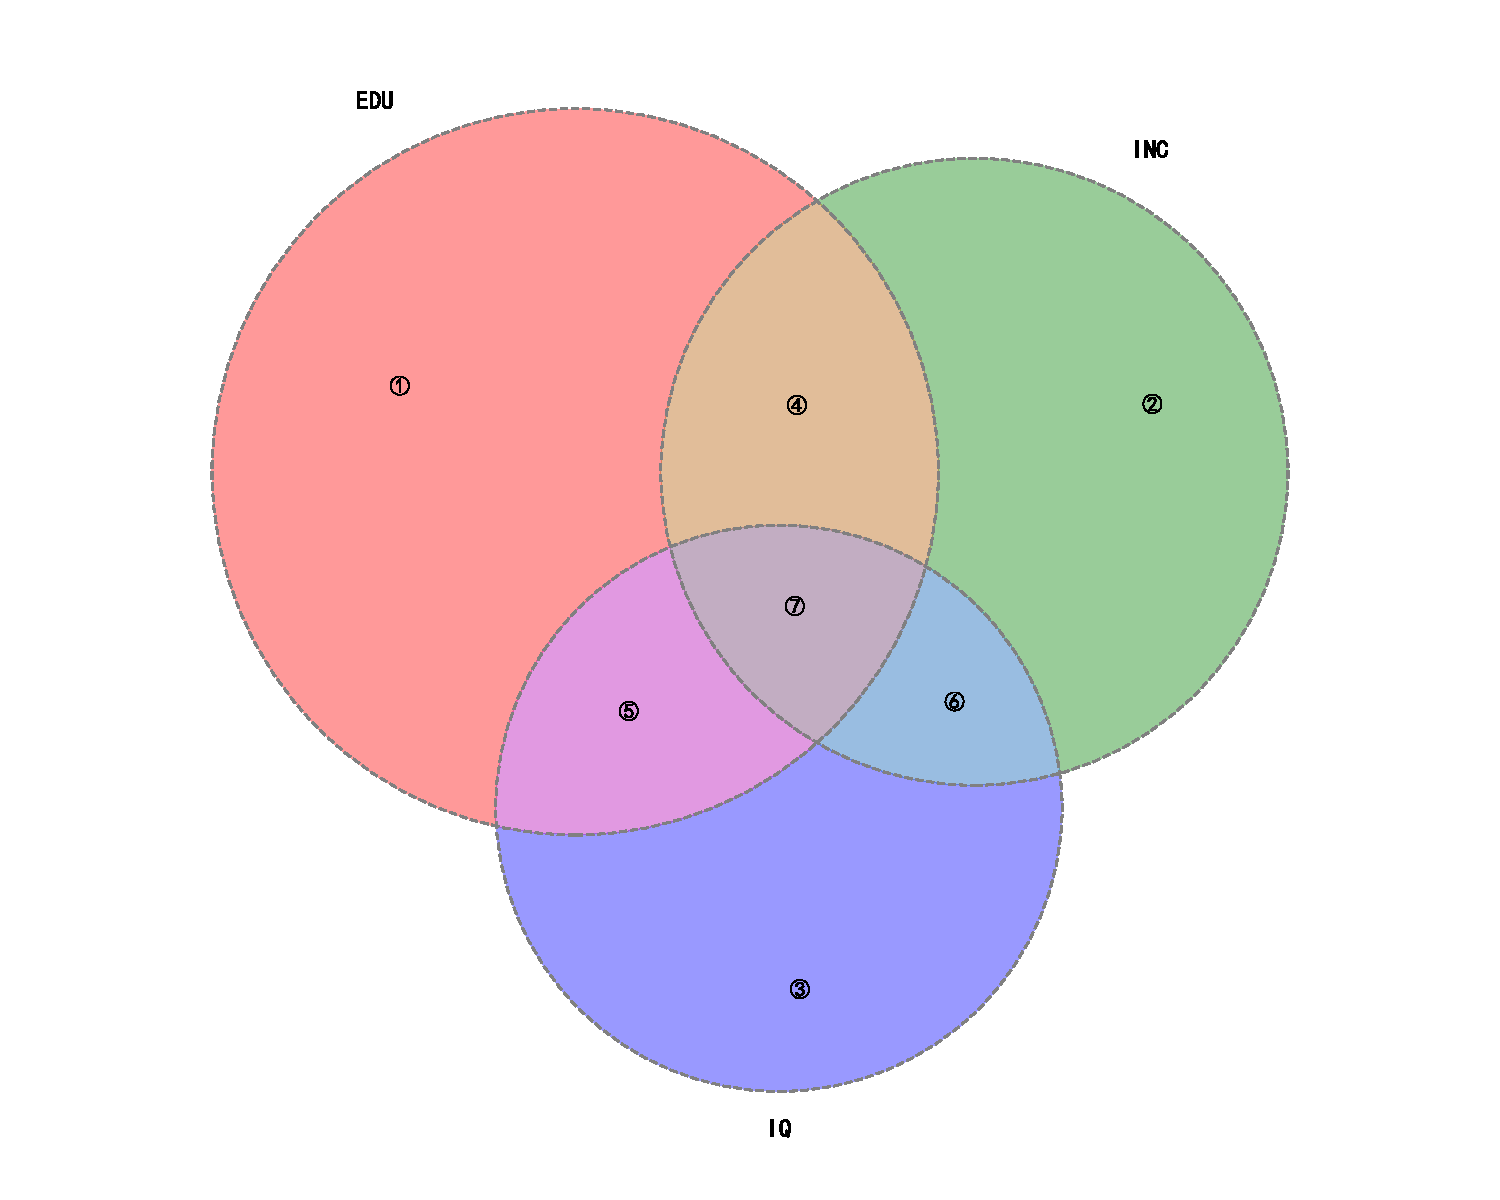
\includegraphics[width=0.5\textwidth]{image/venn_diagrams.pdf}}
	\caption{收入与教育间关系的韦恩图}
	\label{fig:venn}
\end{figure}

在这个图中,我们很清晰地看到,没有一个变量具有超凡脱俗的地位(也就是无法确定哪个是被解释变量,哪个是解释变量)。各个变量之间拥有一部分相互交叉的区域,这构成了其关联的部分,也即统计推断意图找到的参数。同时,还包括处于一些外在的区域,这一部分完全可以归入 $\varepsilon$ ——也就是外部的影响因素之中。

故而统计推断始终面临着的问题便是:\textbf{相关性不等于因果性。}但是,相关始终是因果的一个必要条件。依据惯习,从小样本开始学习较为合适。

\subsection{小样本OLS}

\paragraph*{三大假定}

\textbf{线性假定}
古典线性回归模型(Classical Linear Regression Model,CLRM)可以表示为:

\begin{equation}
Y_i = \beta_1 X_{i1} + \beta_2 X_{i2} + \ldots + \beta_K X_{iK} + \varepsilon_i \quad (i=1,\ldots,n)
\end{equation}

其中,$n$表示样本容量,$X_{ij}$代表第$i$个观测值的第$j$个解释变量($j = 1, \ldots, K$),而$\beta_1, \ldots, \beta_K$则是待估参数(回归系数)。特别地,若模型包含常数项,通常令$X_{i1}=1$。

线性假定的核心含义在于每个解释变量对被解释变量的边际效应为常数。值得注意的是,虽然称为"线性"假定,但模型中可以包含高次项或交互项来处理非线性关系,这仍然被视为满足线性假定。例如,一个模型可以表示为:

\begin{equation}
	Y_i = \beta_1 X_{i1} + \beta_2 X_{i1}^2 + \beta_3 X_{i1}^3 + \beta_4 X_{i2} + \beta_5 X_{i3} + \varepsilon_i \quad (i=1,\ldots,n)
\end{equation}

这是一个包含高次项的模型,其中$X_{i1}$的二次项$X_{i1}^2$和三次项$X_{i1}^3$被引入模型中。尽管模型中包含了变量的高次项,但该模型仍然是线性模型,因为模型关于参数$\beta_1, \beta_2, \ldots, \beta_{5}$是线性的。也就是说,每个参数都以一次方的形式出现,参数之间没有相乘或非线性关系。

在实际应用中,我们可以将$X_{i1}^2$看作一个新的变量$Z_{i1}=X_{i1}^2$,将$X_{i1}^3$看作另一个新变量$Z_{i2}=X_{i1}^3$,这样模型就转化为标准的线性形式:

\begin{equation}
	Y_i = \beta_1 X_{i1} + \beta_2 Z_{i1} + \beta_3 Z_{i2} + \cdots + \varepsilon_i \quad (i=1,\ldots,n)
\end{equation}

因此,只要模型关于参数是线性的,无论变量之间存在怎样的非线性关系,该模型都属于线性回归模型的范畴。

为了更简洁地表达模型,我们定义以下矩阵:
\begin{itemize}
\item $\mathbf{x}_i' = (X_{i1}, X_{i2}, \ldots, X_{iK})$
\item $\boldsymbol{\beta} = (\beta_1, \beta_2, \ldots, \beta_K)'$
\item $\varepsilon_i$表示扰动项
\end{itemize}

单个观测方程可以表示为:
\begin{equation}
Y_i = \mathbf{x}_i' \boldsymbol{\beta} + \varepsilon_i \quad (i=1,\ldots,n) 
\end{equation}

将所有观测方程叠放,我们得到:
\begin{equation}
\mathbf{Y} = \mathbf{X} \boldsymbol{\beta} + \boldsymbol{\varepsilon}
\end{equation}

其中:
\begin{itemize}
\item $\mathbf{Y} = (Y_1, Y_2, \ldots, Y_n)'$
\item $\mathbf{X} = (\mathbf{x}_1, \mathbf{x}_2, \ldots, \mathbf{x}_n)'$是$n \times K$的设计矩阵
\item $\boldsymbol{\varepsilon} = (\varepsilon_1, \varepsilon_2, \ldots, \varepsilon_n)'$是扰动项向量
\end{itemize}

\textbf{严格外生性假定}

严格外生性假定表示为:
\begin{equation}
E(\varepsilon_i | \mathbf{X}) = E(\varepsilon_i | \mathbf{x}_1, \ldots, \mathbf{x}_n) = 0 \quad (i=1,\ldots,n)
\end{equation}

这一假定的含义是,给定数据矩阵$\mathbf{X}$,扰动项的条件期望为零。这意味着$\varepsilon_i$均值独立于所有解释变量的观测数据。由此可以推导出两个重要推论:首先,扰动项的无条件期望也为零,即$E(\varepsilon_i) = 0$;其次,解释变量与扰动项正交,即$Cov(\mathbf{x}_{ik}, \varepsilon_i) = 0$。

如果严格外生性假定被违反,即$E(\varepsilon_i|\mathbf{X}) \neq 0$ 时,将会产生以下后果:

最小二乘估计(Ordinary Least Squares, OLS)将不再是无偏的(unbiased),其推论与统计性质将受到严重影响,主要后果包括:

\begin{enumerate}
\item OLS估计量偏误(Bias):
若扰动项与解释变量存在相关性,OLS估计的系数将系统性偏离真实值,即 $E(\hat{\boldsymbol{\beta}}) \neq \boldsymbol{\beta}$ 。这种偏误不是由样本波动引起的,而是源于模型设定中系统性的信息遗漏或内生性问题。

\item 估计量不再一致(Inconsistency):
在样本容量趋近无穷时,OLS估计也不能收敛于真实参数值,即不满足一致性(consistency)。这意味着收集更多的数据并不能解决偏误问题。

\item 回归结果不可解释为因果效应:
如果解释变量与误差项相关,回归系数不再具有因果解释,因为部分变异源于未被模型控制的系统性因素,因果推断的基础条件——可忽略性(ignorability)或条件独立性——遭到破坏。

\item 推论统计量失效:
OLS估计量的标准误可能低估或高估实际的不确定性,导致 $t$ 检验和 $F$ 检验的显著性水平失真,从而产生虚假显著或遗漏显著变量。
\end{enumerate}

\textbf{为何产生内生性问题(Endogeneity)?}

违反严格外生性假定通常是由于模型中存在遗漏变量(omitted variables)、互为因果(simultaneity)和测量误差(measurement error)等内生性来源,这些问题必须通过其他方法(如工具变量法、双重差分、固定效应模型等)加以处理。


因此,严格外生性是OLS估计可靠性的基石,一旦被违反,必须通过理论论证和实证检验识别偏误来源,并考虑替代的识别策略,这也是统计推断迈向因果推断的关键环节。

\textbf{不存在严格多重共线性假定}

该假定要求数据矩阵$\mathbf{X}$满列秩:
\begin{equation}
	\text{rank}(\mathbf{X}) = K
\end{equation}

如果这一条件不满足,则参数$\boldsymbol{\beta}$不可识别(有趣的案例可见第三章中对KKV三人理论的介绍)。在实际应用中,除非设置过多虚拟变量且包含常数项,否则严格多重共线性的情况较为少见。

满足上述三大假定可以帮助我们实现对方程整体的正确估计,但是,为了确保模型有效性,我们需要考虑残差性质。因而继续引入了更多假定:

\textbf{球型扰动项假定}

球型扰动项假定的矩阵形式为:
\begin{equation}
	Var(\boldsymbol{\varepsilon} | \mathbf{X}) = \sigma^2 \mathbf{I}_n
\end{equation}

其中:
\begin{equation*}
	\boldsymbol{\varepsilon} = 
	\begin{pmatrix}
	\varepsilon_1 \\
	\varepsilon_2 \\
	\vdots \\
	\varepsilon_n
	\end{pmatrix} \quad 
	\mathbf{I}_n = 
	\begin{pmatrix}
	1 & 0 & \cdots & 0 \\
	0 & 1 & \cdots & 0 \\
	\vdots & \vdots & \ddots & \vdots \\
	0 & 0 & \cdots & 1
	\end{pmatrix}
\end{equation*}

这表明误差项向量服从均值为0,协方差矩阵为 $\sigma^2 \mathbf{I}_n$ 的多元正态分布,其中每个误差项的方差都是 $\sigma^2$,且误差项之间互不相关。

这一假定包含两个重要性质:条件同方差性($Var(\varepsilon_i | \mathbf{X}) = \sigma^2$)和无自相关性($Cov(\varepsilon_i, \varepsilon_j | \mathbf{X}) = 0$对于$i \neq j$)。这些性质保证了OLS估计量的有效性,后续我们将考虑违背该假定下的情况以及如何修正。

\paragraph*{如何估计参数?}

回归模型建立之后,我们的首要任务是对模型中的参数进行估计。参数估计的方法主要包括最小二乘估计(Ordinary Least Squares, OLS)、最大似然估计(Maximum Likelihood Estimation, MLE)以及矩估计(Method of Moments)。本节将围绕最为基础且广泛使用的最小二乘估计展开介绍。

\textbf{残差平方和最小化}

在线性回归模型中,最小二乘法的核心思想是使残差平方和(Sum of Squared Residuals, SSR)最小。对于参数的任意假设值$\tilde{\boldsymbol{\beta}}$,我们定义残差向量为:
\begin{equation}
\mathbf{e} = \mathbf{Y} - \mathbf{X}\tilde{\boldsymbol{\beta}}
\end{equation}

最小化的目标函数为残差平方和:
\begin{equation}
	SSR(\tilde{\boldsymbol{\beta}}) = \sum_{i=1}^n e_i^2 = \mathbf{e}'\mathbf{e} = (\mathbf{Y} - \mathbf{X}\tilde{\boldsymbol{\beta}})'(\mathbf{Y} - \mathbf{X}\tilde{\boldsymbol{\beta}})
\end{equation}

展开上述表达式,可得:
\begin{equation}
	SSR(\tilde{\boldsymbol{\beta}}) = \mathbf{Y}'\mathbf{Y} - 2\mathbf{Y}'\mathbf{X}\tilde{\boldsymbol{\beta}} + \tilde{\boldsymbol{\beta}}'\mathbf{X}'\mathbf{X}\tilde{\boldsymbol{\beta}}
\end{equation}

\begin{tcolorbox}[title=使用Stata 中的 auto 数据集进行演示, colback=white, colframe=black, colbacktitle=white, coltitle=black,fonttitle=\bfseries]
	\begin{lstlisting}[xleftmargin=2em, commentstyle=\color{black}]
clear all
quietly sysuse auto, clear

* 我们设定一个简单的小样本回归模型(含截距)
* 以 price 为因变量,mpg, weight, foreign 为解释变量
regress price mpg weight foreign
	\end{lstlisting}
	\vspace{-2em}
	\begin{Verbatim}[commandchars=\\\{\},xleftmargin=2em]

      Source |       SS           df       MS      Number of obs   =        74
-------------+----------------------------------   F(3, 70)        =     23.29
       Model |   317252881         3   105750960   Prob > F        =    0.0000
    Residual |   317812515        70  4540178.78   R-squared       =    0.4996
-------------+----------------------------------   Adj R-squared   =    0.4781
       Total |   635065396        73  8699525.97   Root MSE        =    2130.8

------------------------------------------------------------------------------
       price | Coefficient  Std. err.      t    P>|t|     [95\% conf. interval]
-------------+----------------------------------------------------------------
         mpg |    21.8536   74.22114     0.29   0.769    -126.1758     169.883
      weight |   3.464706    .630749     5.49   0.000     2.206717    4.722695
     foreign |    3673.06   683.9783     5.37   0.000     2308.909    5037.212
       \_cons |  -5853.696   3376.987    -1.73   0.087    -12588.88    881.4934
------------------------------------------------------------------------------
	\end{Verbatim}

\end{tcolorbox}

\textbf{向量微分与正规方程}

利用向量微分规则,对$SSR(\tilde{\boldsymbol{\beta}})$关于$\tilde{\boldsymbol{\beta}}$求导,并令导数为零,即可得到最小值的条件:
\begin{equation}
	\frac{\partial SSR}{\partial \tilde{\boldsymbol{\beta}}} = -2\mathbf{X}'\mathbf{Y} + 2\mathbf{X}'\mathbf{X}\tilde{\boldsymbol{\beta}} = \mathbf{0}
\end{equation}

这便是所谓的正规方程(Normal Equation):
\begin{equation}
	\mathbf{X}'\mathbf{X}\hat{\boldsymbol{\beta}} = \mathbf{X}'\mathbf{Y}
\end{equation}

在$\mathbf{X}'\mathbf{X}$是可逆的前提下(也就是不存在严格的多重共线问题),我们可以求得最小二乘估计量:
\begin{equation}
	\hat{\boldsymbol{\beta}} = (\mathbf{X}'\mathbf{X})^{-1}\mathbf{X}'\mathbf{Y}
\end{equation}

\begin{tcolorbox}[title=在 Stata 的 Mata 中用矩阵(正规方程)显式计算 OLS 解, colback=white, colframe=black, colbacktitle=white, coltitle=black,fonttitle=\bfseries]
	\begin{lstlisting}[xleftmargin=2em, commentstyle=\color{black}]
* 构造设计矩阵 X 与因变量向量 Y(排除缺失)
quietly keep if !missing(price, mpg, weight, foreign)

* 生成常数项并保存数据顺序索引
capture gen double cons = 1
quietly order cons price mpg weight foreign

* 创建 X 矩阵与 Y 向量到 Mata,做矩阵运算
mata:
st_view(Y=., ., "price") // 创建一个指向变量price的视图矩阵Y
st_view(X=., ., ("cons","mpg","weight","foreign")) // 创建指向变量的视图矩阵X
/* 计算 OLS */
b = invsym(X'*X) * (X'*Y)  // 使用正规方程计算OLS估计量:b = (X'X)^(-1)X'Y
b = colshape(b, 1) // 确保b是列向量形式
st_numscalar("n_obs", rows(X)) // 将观测数(X的行数)存储为标量n_obs
b // 显示计算得到的系数向量b
end

* 把 Mata 得到的系数显示与 regress 对比
matrix list e(b)       // 来自 regress 的系数(行向量)
mata: st_matrix("b_mata", b')   // 转成 Stata 矩阵形式(1 x K)
matrix list b_mata
	\end{lstlisting}
	\vspace{-2em}
	\begin{Verbatim}[commandchars=\\\{\},xleftmargin=2em]

. mata:
…… 过程省略
: end

e(b)[1,4]
           mpg      weight     foreign       \_cons
y1   21.853604   3.4647058   3673.0604  -5853.6957

b\_mata[1,4]
            c1          c2          c3          c4
r1   21.853604   3.4647058   3673.0604  -5853.6957
	\end{Verbatim}

\end{tcolorbox}

\textbf{残差性质与方差估计}

估计得出参数后,我们可以计算残差向量$\hat{\mathbf{e}} = \mathbf{Y} - \mathbf{X}\hat{\boldsymbol{\beta}}$。这一残差向量具有与解释变量正交的重要性质,即:
\begin{equation}
\mathbf{X}'\hat{\mathbf{e}} = \mathbf{0}
\end{equation}

这意味着,拟合值$\hat{\mathbf{Y}} = \mathbf{X}\hat{\boldsymbol{\beta}}$与残差$\hat{\mathbf{e}}$在向量空间中正交,两者共同构成了$\mathbf{Y}$的正交分解。

进一步地,我们可以得到误差项方差$\sigma^2$的无偏估计量:
\begin{equation}
	s^2 = \frac{1}{n-K} \sum_{i=1}^n \hat{e}_i^2 = \frac{\hat{\mathbf{e}}'\hat{\mathbf{e}}}{n-K}
\end{equation}

其中$n-K$为自由度,$K$为解释变量(含截距项)个数。标准误差定义为$s = \sqrt{s^2}$,它衡量了残差的离散程度。

\begin{tcolorbox}[title=在 Stata 的 Mata 中计算残差、SSR、$s^2$ 与协方差矩阵、标准误, colback=white, colframe=black, colbacktitle=white, coltitle=black,fonttitle=\bfseries]
	\begin{lstlisting}[xleftmargin=2em, commentstyle=\color{black}]
mata:
/* 重新读取 X,Y,b */
st_view(Y=., ., "price") // 创建指向因变量price的视图矩阵Y
st_view(X=., ., ("mpg","weight","foreign","cons")) // 创建指向自变量的视图矩阵X
b = invsym(X'*X) * (X'*Y) // 使用正规方程计算OLS估计量:b = (X'X)^(-1)X'Y
Yhat = X * b // 计算拟合值:Yhat = X*b
e = Y - Yhat // 计算残差向量:e = Y - Yhat
RSS = e'*e // 计算残差平方和:RSS = e'*e
n = rows(X) // 获取样本数量(观测数)
K = cols(X) // 获取参数个数(变量个数)
s2 = RSS / (n - K) // 计算误差项方差的无偏估计:s² = RSS/(n-K)
s = sqrt(s2) // 计算残差标准差:s = √s²
Vb = s2 * invsym(X'*X) // 计算参数估计量的协方差矩阵:Var(b) = s²(X'X)^(-1)
se = sqrt(diagonal(Vb)) // 提取协方差矩阵对角线元素的平方根得到标准误
/* 输出 */
st_numscalar("RSS", RSS[1,1]) // 将RSS存储为Stata标量
st_numscalar("s2", s2[1,1]) // 将s²存储为Stata标量
st_numscalar("s", s[1,1]) // 将s存储为Stata标量
st_matrix("Vb", Vb) // 将协方差矩阵Vb存储为Stata矩阵
st_matrix("se_b", se') // 将标准误向量存储为Stata矩阵
st_matrix("b_hat", b') // 将参数估计值存储为Stata矩阵
end

display "残差平方和 RSS = " %9.4f RSS
display "误差方差的无偏估计 s^2 = " %9.6f s2
display "残差标准差 s = " %9.6f s
matrix list Vb
matrix list se_b
matrix list b_hat

* 比较 Stata 的 e(V) 与 我们计算的 Vb
matrix list e(V)
* e(V) 和 Vb 数值相同
	\end{lstlisting}

\end{tcolorbox}
\begin{tcolorbox}[title=在 Stata 的 Mata 中计算残差、SSR、$s^2$ 与协方差矩阵、标准误, colback=white, colframe=black, colbacktitle=white, coltitle=black,fonttitle=\bfseries]
	\vspace{-2em}

	\begin{Verbatim}[commandchars=\\\{\},xleftmargin=2em]


. mata:
…… 过程省略
: end

残差平方和 RSS =  3.18e+08
误差方差的无偏估计 s\^{}2 =  4.54e+06
残差标准差 s =  2.13e+03

symmetric Vb[4,4]
            c1          c2          c3          c4
r1   5508.7774
r2     36.2912   .39784425
r3   9089.6431     218.835   467826.27
r4   -229604.2  -2039.2381  -993431.72    11404044

se\_b[1,4]
           c1         c2         c3         c4
r1  74.221139  .63074896  683.97827  3376.9874

b\_hat[1,4]
            c1          c2          c3          c4
r1   21.853604   3.4647058   3673.0604  -5853.6957

symmetric e(V)[4,4]
                mpg      weight     foreign       \_cons
    mpg   5508.7774
 weight     36.2912   .39784425
foreign   9089.6431     218.835   467826.27
  \_cons   -229604.2  -2039.2381  -993431.72    11404044
	\end{Verbatim}

\end{tcolorbox}

\begin{tcolorbox}[title=在 Stata 的 Mata 中验证(残差与解释变量正交), colback=white, colframe=black, colbacktitle=white, coltitle=black, fonttitle=\bfseries]
	\begin{lstlisting}[xleftmargin=2em, commentstyle=\color{black}]
* 先生成常数项
capture gen double cons = 1

* 先预测残差
predict double ehat, resid

* 在 Mata 中读取 X 和 ehat,并计算 X'e
mata:
st_view(X=., ., ("cons","mpg","weight","foreign"))
st_view(e=., ., "ehat")
Xe = X' * e
Xe
end
display "理论上 X' * e = 0,各项应接近 0"
	\end{lstlisting}
	\vspace{-2em}
	\begin{Verbatim}[commandchars=\\\{\},xleftmargin=2em]

. mata:
------------------------------------------------- mata (type end to exit) -----
: st\_view(X=., ., ("cons","mpg","weight","foreign"))
: st\_view(e=., ., "ehat")
: Xe = X' * e
: Xe
                 1
    +---------------+
  1 |  1.16415e-10  |
  2 |  2.11003e-09  |
  3 |  3.42727e-07  |
  4 |  3.63798e-12  |
    +---------------+
: end
-------------------------------------------------------------------------------
理论上 X' * e = 0,各项应接近 0
	\end{Verbatim}

\end{tcolorbox}

\textbf{Frisch--Waugh--Lovell(FWL)定理}

FWL 定理揭示了多元回归中某个变量系数的估计,可以通过“残差回归”的方式得到。设我们有如下的多元线性回归模型:
\begin{equation}
\mathbf{Y} = \mathbf{X}_1 \beta_1 + \mathbf{X}_2 \beta_2 + \boldsymbol{\varepsilon}
\end{equation}

其中 $\mathbf{Y}$ 为 $n \times 1$ 因变量向量,$\mathbf{X}_1$ 为 $n \times k_1$ 的解释变量矩阵,$\mathbf{X}_2$ 为 $n \times k_2$ 的控制变量矩阵。

在多元回归中,$\beta_1$ 衡量的是在控制了 $X_2$ 的影响后,$X_1$ 对 $Y$ 的边际效应。FWL 定理告诉我们,我们可以在不直接进行多元回归的情况下,通过对变量进行“净化”(消去 $X_2$ 的部分)来得到同样的系数估计。

假设我们仅关心 $\beta_1$ 的估计值,可以按以下三步操作:
\begin{enumerate}
	\item 将 $Y$ 对 $X_2$ 回归,取残差 $e_Y$,即
	\begin{equation}
	e_Y = Y - \hat{\alpha}_0 - \hat{\alpha}_2 X_2
	\end{equation}

	\item 将 $X_1$ 对 $X_2$ 回归,取残差 $e_{X_1}$,即
	\begin{equation}
	e_{X_1} = X_1 - \hat{\gamma}_0 - \hat{\gamma}_2 X_2
	\end{equation}

	\item 将 $e_Y$ 对 $e_{X_1}$ 进行一元回归,得到的回归系数即为 $\beta_1$ 的估计值:
	\begin{equation}
	e_Y = \beta_1 e_{X_1} + \text{residual}
	\end{equation}
\end{enumerate}

这种方法的实质是:先用 $X_2$ 消除 $Y$ 与 $X_1$ 中由 $X_2$ 解释的部分,然后在“净化”后的数据之间建立回归关系。

FWL 定理的矩阵证明,$\beta_1$ 的 OLS 估计可以通过如下步骤获得:

\begin{enumerate}
	\item \textbf{对 $\mathbf{Y}$ 回归 $\mathbf{X}_2$,取残差:}
	\begin{equation}
	\mathbf{e}_Y = \mathbf{M}_2 \mathbf{Y}
	\end{equation}

	其中 $\mathbf{M}_2 = \mathbf{I} - \mathbf{P}_2$,$\mathbf{P}_2 = \mathbf{X}_2(\mathbf{X}_2'\mathbf{X}_2)^{-1}\mathbf{X}_2'$ ,其是 $\mathbf{X}_2$ 的投影矩阵。
	\item \textbf{对 $\mathbf{X}_1$ 的每一列回归 $\mathbf{X}_2$,取残差:}
	\begin{equation}
	\mathbf{e}_{X_1} = \mathbf{M}_2 \mathbf{X}_1
	\end{equation}
	
	即对 $\mathbf{X}_1$ 的每一列都做一次“净化”。
	\item \textbf{用 $\mathbf{e}_Y$ 对 $\mathbf{e}_{X_1}$ 做一元或多元回归,得到系数:}
	\begin{equation}
	\hat{\beta}_1 = \left( \mathbf{X}_1'\mathbf{M}_2\mathbf{X}_1 \right)^{-1} \mathbf{X}_1'\mathbf{M}_2\mathbf{Y}
	\end{equation}

	这与直接对 $\mathbf{Y}$ 回归 $\mathbf{X}_1$ 和 $\mathbf{X}_2$ 得到的 $\beta_1$ 完全一致。
\end{enumerate}

$\mathbf{M}_2$ 的作用是将向量投影到与 $\mathbf{X}_2$ 张成空间正交的子空间,即“剔除”了 $\mathbf{X}_2$ 的影响。FWL 定理说明,控制变量的作用就是把因变量和解释变量都净化后再做回归,得到的系数就是多元回归中该变量的边际效应。

FWL 定理的重要意义在于,它为多元回归系数提供了一个分解式解释:\textbf{多元回归中的某个系数等于“净化”该变量与因变量后,两者之间的一元回归系数}。这一结果不仅在理论推导中有用,更为理解控制变量的本质提供了数理上的直观视角。

在韦恩图\ref{fig:venn}中:
\begin{itemize}
    \item INC 与 IQ 的重叠部分⑥⑦表示 IQ 对收入的解释部分;
    \item EDU 与 IQ 的重叠部分⑤⑦表示 IQ 对教育的解释部分。
\end{itemize}

我们通过第一步和第二步回归,分别剔除了 INC 和 EDU 中由 IQ 解释的那一部分(即图中 IQ 与其他圆的重叠部分⑤⑥⑦)

第三步回归实质上是在比较两个“去掉 IQ 影响后的残差”之间的关系,即对应于图中 EDU 与 INC 在 IQ 之外的交集区域(也就是④)。

\begin{tcolorbox}[title=在 Stata 中展示FWL定理, colback=white, colframe=black, colbacktitle=white, coltitle=black,fonttitle=\bfseries]
	\begin{lstlisting}[xleftmargin=2em, commentstyle=\color{black}]
* 目标:展示在控制 weight, foreign 时 mpg 的系数
* 等同于:先对 price 与 mpg 分别“剔除” weight & foreign 的影响,再做一元回归
* 先看完整模型中 mpg 的估计系数(已在 regress 输出)
quietly regress price mpg weight foreign
local b1 = _b[mpg]
display "多元回归中 mpg 的系数 = " %9.6f `b1'
* 第一步:price 对 weight foreign 回归,取残差 eY
quietly regress price weight foreign
capture predict double eY, resid
* 第二步:mpg 对 weight foreign 回归,取残差 eX1
quietly regress mpg weight foreign
capture predict double eX1, resid
* 第三步:用 eY 对 eX1 做一元回归
quietly regress eY eX1
local b2 = _b[eX1]
display "用 eY 对 eX1 做一元回归得到的系数 = " %9.6f `b2'
* 第四步:进一步讨论 FWL 定理
quietly regress price eX1
local b3 = _b[eX1]
display "用 Y 对 eX1 做一元回归得到得到的系数 = " %9.6f `b3'
* 第五步:进一步讨论 FWL 定理
quietly regress eY mpg weight foreign
local b4 = _b[mpg]
display "用 eY 对 mpg 做多元回归得到得到的系数 = " %9.6f `b4'
	\end{lstlisting}
	\vspace{-2em}
	\begin{Verbatim}[commandchars=\\\{\},xleftmargin=2em]

多元回归中 mpg 的系数 = 21.853604
用 eY 对 eX1 做一元回归得到的系数 = 21.853604
用 Y 对 eX1 做一元回归得到得到的系数 = 21.853604
用 eY 对 mpg 做多元回归得到得到的系数 = 21.853604
	\end{Verbatim}

\end{tcolorbox}

图\ref{fig:venncol}表示的是一个高度共线情况下的韦恩图,从图中我们可以看到,IQ 与 INC 的重叠部分⑥⑦表示 IQ 对收入的解释部分;IQ 与 EDU 的重叠部分⑤⑦表示 IQ 对教育的解释部分。在剔除IQ影响后的残差之间进行一元回归,得到的回归系数即为 EDU 的估计值,但是由于这一部分过于庞大,因此我们无法从结果中得到有效的解释。

\begin{figure}[ht]
	\centering
	\fbox{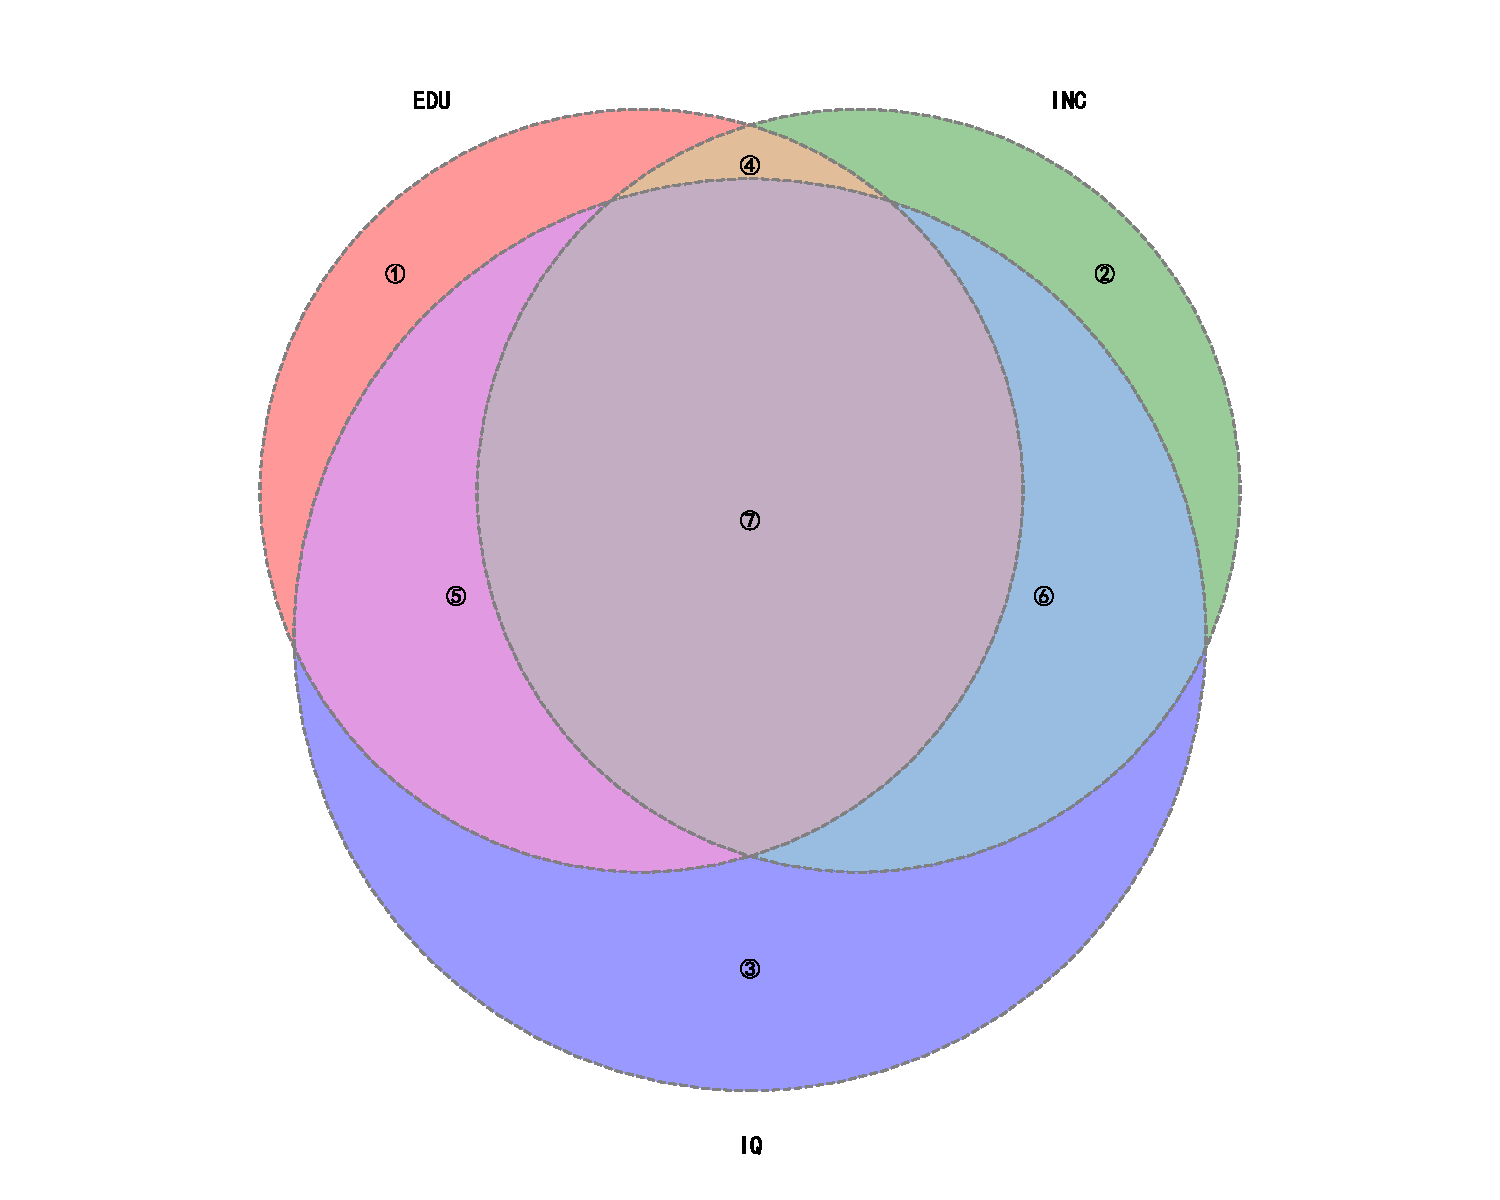
\includegraphics[width=0.5\textwidth]{image/venn_diagrams_collinearity.pdf}}
	\caption{高度共线下的韦恩图}
	\label{fig:venncol}
\end{figure}

\newpage

\textbf{平方和分解与拟合优度}

若模型中包含常数项,我们可以建立响应变量的平方和分解:
\begin{equation}
	\sum_{i=1}^n (Y_i - \bar{Y})^2 = \sum_{i=1}^n (\hat{Y}_i - \bar{Y})^2 + \sum_{i=1}^n \hat{e}_i^2
\end{equation}

其中,左侧为总离差平方和(Total Sum of Squares, TSS),右侧第一项为回归平方和(Explained Sum of Squares, ESS),第二项为残差平方和(Residual Sum of Squares, RSS)。据此定义拟合优度$R^2$为:
\begin{equation}
	R^2 = \frac{ESS}{TSS} = 1 - \frac{RSS}{TSS}
\end{equation}

该指标反映了模型解释总变异的能力,其数值介于0与1之间,越接近1表示模型拟合越好。该指标在多数统计软件中会自动给出,用以反映无截距模型的拟合程度。

通俗地说,我们可以将总变异(TSS)理解为数据的"总信息量",它被分解为两部分:
\begin{itemize}
\item 由模型解释的部分(ESS):这是我们通过自变量能够捕捉到的"有用信息"
\item 未被模型解释的部分(RSS):这是模型无法解释的"剩余信息"或"噪音"
\end{itemize}

$R^2$就像一个"信息利用率"指标,告诉我们模型能够解释多少比例的数据变异。例如,$R^2=0.5$意味着模型能够解释因变量中50\%的变异。

需要注意的是,简单地增加变量数量通常会使$R^2$增大,但这并不意味着模型质量提高。为了惩罚变量过多可能导致的虚高$R^2$,我们引入校正拟合优度$\bar{R}^2$(Adjusted $R^2$),校正后的$R^2$考虑了模型复杂度,只有当新增变量带来的信息增益超过其增加的复杂度时,$\bar{R}^2$才会增加:

\begin{equation}
	\bar{R}^2 = 1 - \frac{RSS/(n-K)}{TSS/(n-1)} = 1 - \frac{n-1}{n-K}(1-R^2)
\end{equation}

在\textbf{机器学习(ML)}中,$R^2$ 往往被视为预测精度的重要度量之一,其优化目标是尽可能减少预测误差。然而在因果推断中,研究者的核心关注点并非预测准确,而是获得对处理效应(treatment effect)的无偏、可解释估计值。一个因果模型即便 $R^2$ 较低,只要能够正确识别出因果效应,也具有高度学术价值;反之,一个 $R^2$ 极高但因果识别错误的模型,在政策建议或理论解释上可能毫无意义,故而社会科学范式中对于 $R^2$ 的考量往往并不严格。

\begin{tcolorbox}[title={在 Stata 的 Mata 中进行平方和分解($TSS = ESS + RSS$)与 $R^2$ 计算}, colback=white, colframe=black, colbacktitle=white, coltitle=black, fonttitle=\bfseries]
	\begin{lstlisting}[xleftmargin=2em, commentstyle=\color{black}]
* 计算 TSS, ESS, RSS 并核对 R^2
summarize price, meanonly // 计算price变量的均值
scalar Ybar = r(mean) // 将price的均值存储为标量Ybar
quietly regress price mpg weight foreign // 静默运行回归(不显示结果)
scalar b_cons = _b[_cons] // 提取并存储常数项系数
scalar b_mpg = _b[mpg] // 提取并存储mpg变量的系数
scalar b_weight = _b[weight] // 提取并存储weight变量的系数
scalar b_foreign = _b[foreign] // 提取并存储foreign变量的系数
capture generate double Yhat = b_cons + b_mpg*mpg + b_weight*weight + b_foreign*foreign
// 根据系数计算拟合值Yhat
capture generate double resid = price - Yhat // 计算残差值(实际值减去拟合值)
quietly summarize price, detail // 静默计算price的详细统计信息

mata:
st_view(Y=., ., "price") // 创建指向price变量的视图矩阵Y
st_view(Yhat=., ., "Yhat") // 创建指向Yhat变量的视图矩阵Yhat
st_view(resid=., ., "resid") // 创建指向resid变量的视图矩阵resid
TSS = (Y :- mean(Y))' * (Y :- mean(Y)) // 计算总离差平方和TSS = Σ(yi - ȳ)²
ESS = (Yhat :- mean(Y))' * (Yhat :- mean(Y)) // 计算回归平方和ESS = Σ(ŷi - ȳ)²
RSS = resid' * resid // 计算残差平方和RSS = Σ(êi)²
st_numscalar("TSS_s", TSS[1,1]) // 将TSS存储为Stata标量
st_numscalar("ESS_s", ESS[1,1]) // 将ESS存储为Stata标量
st_numscalar("RSS_s", RSS[1,1]) // 将RSS存储为Stata标量
end

display "TSS = " %9.4f scalar(TSS_s)
display "ESS = " %9.4f scalar(ESS_s)
display "RSS = " %9.4f scalar(RSS_s)
display "TSS - ESS - RSS = " %9.8f (scalar(TSS_s) - scalar(ESS_s) - scalar(RSS_s))
display "R^2 = " %9.6f (scalar(ESS_s) / scalar(TSS_s))
	\end{lstlisting}
	\vspace{-2em}
	\begin{Verbatim}[commandchars=\\\{\},xleftmargin=2em]

. mata:
…… 过程省略
: end
TSS =  6.35e+08
ESS =  3.17e+08
RSS =  3.18e+08
TSS - ESS - RSS = -0.00000036
R\^{}2 =  0.499559
	\end{Verbatim}

\end{tcolorbox}

\paragraph*{小样本下OLS估计的基本性质}
小样本下的OLS性质主要包括以下几个方面:

\textbf{线性}
    
    OLS估计量是被解释变量$\mathbf{y}$的线性组合:
    \begin{equation}
        \mathbf{b} = (\mathbf{X}^{\prime}\mathbf{X})^{-1}\mathbf{X}^{\prime}\mathbf{y}
    \end{equation}

\textbf{无偏性}
    
    在古典线性回归模型(CLRM)的假定下(严格外生性、无多重共线性、球型扰动项),OLS估计量是无偏的:
    \begin{equation}
        \operatorname{E}(\mathbf{b} \mid \mathbf{X}) = \boldsymbol{\beta}
    \end{equation}
    即$\mathbf{b}$不会系统性地高估或低估真实参数$\boldsymbol{\beta}$。无偏性的证明依赖于严格外生性假定:
    \begin{equation}
        \operatorname{E}(\epsilon_i \mid \mathbf{X}) = 0
    \end{equation}

\textbf{有效性(高斯-马尔可夫定理)}
    
    在CLRM假定下,OLS估计量是所有线性无偏估计量中方差最小的(BLUE)。即对于任意其他线性无偏估计量$\tilde{\boldsymbol{\beta}}$,有:
    \begin{equation}
        \operatorname{Var}(\tilde{\boldsymbol{\beta}} \mid \mathbf{X}) \geq \operatorname{Var}(\mathbf{b} \mid \mathbf{X})
    \end{equation}

\textbf{正态性与统计检验}
    
    若进一步假设扰动项$\epsilon_i$服从正态分布,则:
    \begin{itemize}
        \item OLS估计量$\mathbf{b}$服从多元正态分布。
        \item 对单个系数的$t$检验和对线性假设的$F$检验在小样本下严格成立(见后文)。
    \end{itemize}

\textbf{局限性}
    \begin{itemize}
        \item 严格外生性:要求解释变量与所有扰动项(过去、现在、未来)均不相关,时间序列中可能不成立。
        \item 正态性假设:若扰动项非正态,小样本下$t/F$检验可能失效,需依赖大样本理论。
        \item 异方差或自相关:若球型扰动项假定不成立,OLS虽无偏但不再有效,需使用GLS或稳健标准误。
    \end{itemize}

小样本下,OLS在CLRM假定下具有无偏性、有效性和正态性,是统计推断的基础。但实际应用中需谨慎检验假定(如异方差、自相关、内生性),必要时转向大样本理论或替代估计方法(如工具变量、GMM)。

\paragraph*{模型检验与预测}

在获得参数估计值之后,我们通常还需对模型的显著性进行检验,并评估模型在未来观测上的预测能力。本节将围绕线性回归模型中的方差估计、假设检验和预测方法进行介绍。

\textbf{方差估计}

如前所述,$s^2$是误差项方差$\sigma^2$的无偏估计量。这一结论基于矩阵迹(trace)运算的性质,具体地:
\begin{equation}
	E(\hat{\mathbf{e}}'\hat{\mathbf{e}} \mid \mathbf{X}) = \sigma^2 \cdot \text{trace}(\mathbf{M}) = \sigma^2 (n - K)
\end{equation}

因此,我们可得参数估计量$\hat{\boldsymbol{\beta}}$的协方差矩阵估计为:
\begin{equation}
	\widehat{\text{Var}}(\hat{\boldsymbol{\beta}} \mid \mathbf{X}) = s^2 (\mathbf{X}'\mathbf{X})^{-1}
\end{equation}

该协方差矩阵为后续进行假设检验和置信区间构建提供了基础。

\textbf{单个系数的检验}

在经典回归模型中,若我们进一步假定扰动项服从正态分布,即$\boldsymbol{\varepsilon} \sim \mathcal{N}(0, \sigma^2 \mathbf{I}_n)$,则参数估计量$\hat{\boldsymbol{\beta}}$亦服从正态分布。

此时,可对任一系数$\beta_k$构造t统计量进行假设检验:
\begin{equation}
	t_k = \frac{\hat{\beta}_k - \beta_k^0}{SE(\hat{\beta}_k)} \sim t(n-K)
\end{equation}

其中$\beta_k^0$为原假设下的理论值,$SE(\hat{\beta}_k)$为对应系数的标准误。我们可以通过计算$t_k$的值,并查阅$t$分布临界值或计算$p$值,判断该系数是否显著不同于零。

此外,置信区间的构建亦基于$t$分布,例如$(1-\alpha)$置信区间为:
\begin{equation}
\hat{\beta}_k \pm t_{\alpha/2}(n-K) \cdot SE(\hat{\beta}_k)
\end{equation}

通俗地说,t分布帮助我们判断回归系数的显著性。t统计量实际上是"信号"与"噪声"的比值:
\begin{itemize}
\item 分子$\hat{\beta}_k - \beta_k^0$代表我们观察到的"信号"(即实际效应与假设值的差异)
\item 分母$SE(\hat{\beta}_k)$代表"噪声"(即估计的不确定性)
\end{itemize}

当t值较大时,说明信号远大于噪声,我们更有信心认为该系数显著不为零。当样本量较小时,t分布比正态分布更"厚尾",能更好地反映小样本的不确定性。

\begin{tcolorbox}[title=在 Stata 的 Mata 中进行单个系数 t 检验, colback=white, colframe=black, colbacktitle=white, coltitle=black,fonttitle=\bfseries]
	\begin{lstlisting}[xleftmargin=2em, commentstyle=\color{black}]
* 检验 mpg 的显著性
* t_k = (b_k - 0) / se(b_k)
matrix list se_b // 列出之前计算的标准误矩阵se_b
mata:
b = st_matrix("b_mata")' // 从Stata矩阵中读取系数估计值,1xK转置为Kx1列向量
se = st_matrix("se_b")' // 从Stata矩阵中读取标准误,1xK转置为Kx1列向量
// 找到 mpg 在第2个位置 (mpg, weight, foreign, cons)
b_mpg = b[1] // 提取mpg变量的系数估计值(第1个位置)
se_mpg = se[1] // 提取mpg变量的标准误(第1个位置)
n = st_numscalar("n_obs") // 从Stata标量中读取样本数量n
K = 4 // 设置参数个数K=4
df = n - K // 计算自由度df = n - K
t_mpg = (b_mpg - 0) / se_mpg // 计算mpg系数的t统计量(原假设为0)
pval = 2 * ttail(df, abs(t_mpg)) // 计算双侧检验的p值(使用t分布的尾部概率)
st_numscalar("t_mpg", t_mpg) // 将计算得到的t统计量存储为Stata标量
st_numscalar("p_mpg", pval) // 将计算得到的p值存储为Stata标量
end

display "t = " %9.4f t_mpg ", p-value = " %9.6f p_mpg " (df = " (n_obs - 4) ")"
	\end{lstlisting}
	\vspace{-2em}
	\begin{Verbatim}[commandchars=\\\{\},xleftmargin=2em]

b\_mata[1,4]
            c1          c2          c3          c4
r1   21.853604   3.4647058   3673.0604  -5853.6957

se\_b[1,4]
           c1         c2         c3         c4
r1  74.221139  .63074896  683.97827  3376.9874

. mata:
…… 过程省略
: end

t =    0.2944, p-value =  0.769294 (df = 70)
	\end{Verbatim}

\end{tcolorbox}

\textbf{线性假设的检验}

当我们希望同时检验多个参数是否满足一组线性约束关系时,可以使用F检验方法。设原假设为:
\begin{equation}
H_0: \mathbf{R}\boldsymbol{\beta} = \mathbf{r}
\end{equation}

其中$\mathbf{R}$为$m \times K$的约束矩阵,$\mathbf{r}$为$m \times 1$的向量。

对应的F统计量为:
\begin{equation}
	F = \frac{(\mathbf{R}\hat{\boldsymbol{\beta}} - \mathbf{r})'[\mathbf{R}(\mathbf{X}'\mathbf{X})^{-1}\mathbf{R}']^{-1}(\mathbf{R}\hat{\boldsymbol{\beta}} - \mathbf{r}) / m}{s^2} \sim F(m, n - K)
\end{equation}

此统计量衡量在给定约束下估计结果偏离原假设的程度,也可通过约束模型与无约束模型的残差平方和之差加以表述,常用于方差分析框架中。

\begin{tcolorbox}[title=在 Stata 的 Mata 中进行线性约束的 F 检验, colback=white, colframe=black, colbacktitle=white, coltitle=black,fonttitle=\bfseries]
	\begin{lstlisting}[xleftmargin=2em, commentstyle=\color{black}]
*  H0: mpg = 0、foreign = 0 和 weight = 0 同时成立
test mpg foreign weight  // 使用Stata内置命令进行F检验

* 先估计无约束(完整)模型,保存 RSS、n、df_r(残差自由度)
quietly regress price mpg weight foreign // 估计包含所有变量的无约束模型
scalar RSS_ur = e(rss) // 保存无约束模型的残差平方和
scalar n_obs  = e(N) // 保存样本数量
scalar df_r   = e(df_r) // 保存残差自由度 = n - k
scalar k      = n_obs - df_r // 计算参数总数(含常数项)

* 再估计受限模型,保存 RSS
quietly regress price // 估计受限模型(仅包含常数项)
scalar RSS_r = e(rss) // 保存受限模型的残差平方和

* 约束数 q = 3 (mpg=0, foreign=0, weight = 0)
scalar q = 3 // 设置约束条件个数

* 根据F统计量公式手动计算 F 值
scalar Fstat = ((RSS_r - RSS_ur)/q) / ( RSS_ur / (n_obs - k) )
display "手动计算 Fstat = " %9.4f Fstat // 显示手动计算的F统计量
	\end{lstlisting}
	\vspace{-2em}
	\begin{Verbatim}[commandchars=\\\{\},xleftmargin=2em]

 ( 1)  mpg = 0
 ( 2)  foreign = 0
 ( 3)  weight = 0

       F(  3,    70) =   23.29
            Prob > F =    0.0000
手动计算 Fstat =   23.2922
	\end{Verbatim}

\end{tcolorbox}

\textbf{点预测与区间预测}

线性回归模型的另一重要应用是进行预测。对于一个新观测,其解释变量为$\mathbf{x}_0'$($1 \times K$行向量),则响应变量的点预测值为:
\begin{equation}
	\hat{Y}_0 = \mathbf{x}_0' \hat{\boldsymbol{\beta}}
\end{equation}

然而,该点预测存在不确定性,主要来源于两方面:一是回归系数估计的误差,二是新样本本身的随机扰动。因此,预测误差的方差为:
\begin{equation}
\text{Var}(\hat{Y}_0 - Y_0) = \sigma^2 + \sigma^2 \cdot \mathbf{x}_0'(\mathbf{X}'\mathbf{X})^{-1}\mathbf{x}_0
\end{equation}

据此,可以构建预测区间:
\begin{equation}
	\left[ \hat{Y}_0 \pm t_{\alpha/2}(n-K) \cdot s \cdot \sqrt{1 + \mathbf{x}_0'(\mathbf{X}'\mathbf{X})^{-1}\mathbf{x}_0} \right]
\end{equation}

该区间既考虑了参数估计的不确定性,也囊括了未来观测点的随机波动,是实际应用中不可或缺的分析工具。

\begin{tcolorbox}[title=在 Stata 的 Mata 中进行点预测与区间预测, colback=white, colframe=black, colbacktitle=white, coltitle=black,fonttitle=\bfseries]
	\begin{lstlisting}[xleftmargin=2em, commentstyle=\color{black}]
* x0 = (1, mpg=25, weight=3000, foreign=0)时Y的预测值和预测区间
mata:
st_view(X=., ., ("cons","mpg","weight","foreign")) // 创建设计矩阵视图
st_view(Y=., ., "price") // 创建因变量视图
b = invsym(X'*X) * (X'*Y) // 计算OLS估计量
x0 = (1, 25, 3000, 0)' // 定义新观测点的变量值
Yhat0 = x0' * b // 计算点预测值
s2 = ((Y - X*b)' * (Y - X*b)) / (rows(X) - cols(X)) // 计算误差方差估计
Vb = s2 * invsym(X'*X) // 计算参数协方差矩阵
var_hatY0 = (x0' * Vb * x0)[1,1] // 计算预测值方差
var_pred  = s2[1,1] + var_hatY0 // 计算预测误差方差
df = rows(X) - cols(X) // 计算自由度
tcrit = invttail(df, 0.025) // 计算95%置信水平的临界值
lower = Yhat0[1,1] - tcrit*sqrt(var_pred) // 计算预测区间下限
upper = Yhat0[1,1] + tcrit*sqrt(var_pred) // 计算预测区间上限
st_numscalar("Yhat0",   Yhat0[1,1]) // 存储点预测值
st_numscalar("pred_se", sqrt(var_pred)) // 存储预测标准误
st_numscalar("tcrit",   tcrit) // 存储临界值
st_numscalar("lower",   lower) // 存储区间下限
st_numscalar("upper",   upper) // 存储区间上限
end

display "点预测 Yhat = " %9.4f scalar(Yhat0) // 显示点预测值
display "预测标准误 = " %9.4f scalar(pred_se) // 显示预测标准误
display "95% 预测区间 = [" %9.4f scalar(lower) ", " %9.4f scalar(upper) "]"  // 显示预测区间
	\end{lstlisting}
	\vspace{-2em}
	\begin{Verbatim}[commandchars=\\\{\},xleftmargin=2em]

. mata:
…… 过程省略
: end

点预测 Yhat = 5086.7619
预测标准误 = 2166.9906
95\% 预测区间 = [ 764.8355, 9408.6884]
	\end{Verbatim}

\end{tcolorbox}

\subsection{大样本与异方差问题}

\paragraph*{大数定律与中心极限定理}

到目前为止,我们已经推导出 $\hat{\boldsymbol{\beta}}$ 的显式表达式,并掌握了其标准误的计算方法。然而,这仅仅完成了估计阶段——就像在一次抽样中观察到某个比例,我们还无法直接判断这一比例是否具有统计显著性。为了检验回归系数是否显著偏离零,我们必须运用\textbf{假设检验}。

在小样本的 OLS 推断中,为了获得系数统计量的精确抽样分布,通常假设随机误差项服从正态分布,从而可直接利用正态分布的性质(或其推导出的 $t$ 与 $F$ 分布)进行假设检验。然而,假设检验的核心问题在于:如果我们能够反复从总体中抽取样本,$\hat{\boldsymbol{\beta}}$ 这一随机变量的抽样分布会呈现怎样的形状?

此时,大数定律和中心极限定理发挥了关键作用。大数定律(Law of Large Numbers, LLN)表明,在适当的条件下,样本矩会收敛到相应的总体矩。具体而言,对于独立同分布的随机变量序列,样本均值将以概率1收敛到总体均值。在OLS估计中,这保证了设计矩阵的样本二阶矩 $\frac{1}{n}\mathbf{X}'\mathbf{X}$ 收敛到其期望值 $\mathrm{E}(\mathbf{x}_i\mathbf{x}_i')$,从而确保了OLS估计量的一致性。

中心极限定理(Central Limit Theorem, CLT)则更进一步——它表明,在误差项独立同分布且方差有限的条件下,即便总体分布形态再复杂,只要样本量足够大,$\hat{\boldsymbol{\beta}}$ 的抽样分布都会趋近于正态分布。这是因为 $\hat{\boldsymbol{\beta}}$ 可表示为多个独立随机变量的加权平均,而加权平均在大样本条件下会"自动"逼近正态分布。这一结果正是大样本推断的理论基石。

换言之,中心极限定理为我们提供了一个正态分布的"模具",可以将抽样得到的系数放入其中,再使用标准化的 $t$ 检验或 $z$ 检验判断它是否显著不为零。

陈强老师的《高级计量经济学及Stata应用(第二版)》中给出了大数定律和中心极限定理在OLS估计中的应用,我们对这部分进行了一个简化:

\begin{theorem}[大样本OLS估计量的渐近正态性]
在满足以下正则条件的线性回归模型中:
\begin{equation}
\mathbf{y} = \mathbf{X}\beta + \mathbf{u}
\end{equation}
其中:
\begin{itemize}
    \item $\mathbf{X}$ 为 $n \times k$ 设计矩阵,$\beta$ 为 $k \times 1$ 参数向量;
    \item 误差项 $\mathbf{u}$ 满足条件外生性:$\mathbb{E}(\mathbf{u}|\mathbf{X}) = 0$;
    \item 同方差性:$\text{Var}(\mathbf{u}|\mathbf{X}) = \sigma^2 \mathbf{I}_n$;
    \item 解释变量满足遍历平稳性与矩存在性,使得 $\frac{1}{n} \sum_{i=1}^n \mathbf{x}_i \mathbf{x}_i^\top \overset{p}{\to} \mathbf{Q}$,其中 $\mathbf{Q}$ 为正定矩阵;
    \item 误差项与解释变量构成的序列 $\{\mathbf{x}_i u_i\}$ 满足中心极限定理条件;
\end{itemize}

则普通最小二乘法(OLS)估计量:
\begin{equation}
\hat{\beta} = (\mathbf{X}^\top \mathbf{X})^{-1} \mathbf{X}^\top \mathbf{y} = \beta + (\mathbf{X}^\top \mathbf{X})^{-1} \mathbf{X}^\top \mathbf{u}
\end{equation}
具有渐近正态性,即:
\begin{equation}
\sqrt{n}(\hat{\beta} - \beta) \overset{d}{\to} N(0, \sigma^2 \mathbf{Q}^{-1})
\end{equation}
从而:
\begin{equation}
\hat{\beta} \overset{a}{\sim} N\left( \beta, \frac{\sigma^2}{n} \mathbf{Q}^{-1} \right)
\end{equation}
其中 $\mathbf{Q} = \mathbb{E}[\mathbf{x}_i \mathbf{x}_i^\top]$,$\overset{a}{\sim}$ 表示"渐近服从"。
\end{theorem}

\begin{proof}
\begin{flushleft}
第一步:标准化估计量的表达式
\end{flushleft}
\begin{flushleft}
由OLS估计量的线性性质,有:
\end{flushleft}
\begin{equation}
\hat{\beta} - \beta = (\mathbf{X}^\top \mathbf{X})^{-1} \mathbf{X}^\top \mathbf{u}
\end{equation}
两边左乘 $\sqrt{n}$ 得到:
\begin{equation}
\sqrt{n}(\hat{\beta} - \beta) = \sqrt{n} (\mathbf{X}^\top \mathbf{X})^{-1} \mathbf{X}^\top \mathbf{u}
\end{equation}
进一步分解为:
\begin{equation}
\sqrt{n}(\hat{\beta} - \beta) = \left( \frac{\mathbf{X}^\top \mathbf{X}}{n} \right)^{-1} \cdot \frac{\mathbf{X}^\top \mathbf{u}}{\sqrt{n}}
\end{equation}
第二步:应用大数定律(LLN)
\begin{flushleft}
定义 $\mathbf{Q}_n = \frac{1}{n} \sum_{i=1}^n \mathbf{x}_i \mathbf{x}_i^\top = \frac{\mathbf{X}^\top \mathbf{X}}{n}$。根据大数定律,在适当平稳性和矩条件下:
\end{flushleft}
\begin{equation}
\mathbf{Q}_n \overset{p}{\to} \mathbf{Q} = \mathbb{E}[\mathbf{x}_i \mathbf{x}_i^\top]
\end{equation}
由于矩阵求逆是连续函数,根据连续映射定理:
\begin{equation}
\left( \frac{\mathbf{X}^\top \mathbf{X}}{n} \right)^{-1} = \mathbf{Q}_n^{-1} \overset{p}{\to} \mathbf{Q}^{-1}
\end{equation}
第三步:应用中心极限定理(CLT)
\begin{flushleft}
定义 $\mathbf{z}_i = \mathbf{x}_i u_i$,则:
\end{flushleft}
\begin{equation}
\frac{\mathbf{X}^\top \mathbf{u}}{\sqrt{n}} = \frac{1}{\sqrt{n}} \sum_{i=1}^n \mathbf{z}_i
\end{equation}
由外生性 $\mathbb{E}[u_i|\mathbf{x}_i] = 0$,得:
\begin{equation}
\mathbb{E}[\mathbf{z}_i] = \mathbb{E}[\mathbf{x}_i u_i] = \mathbb{E}[\mathbf{x}_i \mathbb{E}[u_i|\mathbf{x}_i]] = 0
\end{equation}
在同方差假设下,$\text{Var}(u_i|\mathbf{x}_i) = \sigma^2$,因此:
\begin{equation}
\text{Var}(\mathbf{z}_i) = \mathbb{E}[\mathbf{x}_i \mathbf{x}_i^\top u_i^2] = \mathbb{E}\big[\mathbb{E}[\mathbf{x}_i \mathbf{x}_i^\top u_i^2 \mid \mathbf{x}_i]\big] = \mathbb{E}[\mathbf{x}_i \mathbf{x}_i^\top \mathbb{E}[u_i^2 \mid \mathbf{x}_i]] = \sigma^2 \mathbb{E}[\mathbf{x}_i \mathbf{x}_i^\top] = \sigma^2 \mathbf{Q}
\end{equation}
若 $\{\mathbf{z}_i\}$ 满足CLT条件(如独立同分布或弱相关),则:
\begin{equation}
\frac{1}{\sqrt{n}} \sum_{i=1}^n \mathbf{z}_i \overset{d}{\to} N(0, \sigma^2 \mathbf{Q})
\end{equation}
第四步:应用Slutsky定理
\begin{flushleft}
我们已知:
\end{flushleft}
\begin{itemize}
    \item $\left( \frac{\mathbf{X}^\top \mathbf{X}}{n} \right)^{-1} \overset{p}{\to} \mathbf{Q}^{-1}$;
    \item $\frac{\mathbf{X}^\top \mathbf{u}}{\sqrt{n}} \overset{d}{\to} N(0, \sigma^2 \mathbf{Q})$;
\end{itemize}
\begin{flushleft}
根据Slutsky定理(若 $A_n \overset{p}{\to} A$,$B_n \overset{d}{\to} B$,则 $A_n B_n \overset{d}{\to} AB$),有:
\end{flushleft}
\begin{equation}
\sqrt{n}(\hat{\beta} - \beta) = \left( \frac{\mathbf{X}^\top \mathbf{X}}{n} \right)^{-1} \cdot \frac{\mathbf{X}^\top \mathbf{u}}{\sqrt{n}} \overset{d}{\to} \mathbf{Q}^{-1} \cdot N(0, \sigma^2 \mathbf{Q})
\end{equation}
由于线性变换保持正态性,且:
\begin{equation}
\text{Var}(\mathbf{Q}^{-1} \cdot N(0, \sigma^2 \mathbf{Q})) = \mathbf{Q}^{-1} (\sigma^2 \mathbf{Q}) \mathbf{Q}^{-1} = \sigma^2 \mathbf{Q}^{-1}
\end{equation}
因此:
\begin{equation}
\sqrt{n}(\hat{\beta} - \beta) \overset{d}{\to} N(0, \sigma^2 \mathbf{Q}^{-1})
\end{equation}
第五步:最终渐近分布
\begin{flushleft}
将上式标准化后除以 $\sqrt{n}$,可得:
\end{flushleft}
\begin{equation}
\hat{\beta} - \beta \overset{d}{\to} N\left(0, \frac{\sigma^2}{n} \mathbf{Q}^{-1} \right)
\end{equation}
即:
\begin{equation}
\hat{\beta} \overset{a}{\sim} N\left( \beta, \frac{\sigma^2}{n} \mathbf{Q}^{-1} \right)
\end{equation}

\end{proof}

结论:在大样本条件下,OLS估计量 $\hat{\beta}$ 是渐近正态的,其渐近协方差矩阵为 $\frac{\sigma^2}{n} \mathbf{Q}^{-1}$,其中 $\mathbf{Q} = \mathbb{E}[\mathbf{x}_i \mathbf{x}_i^\top]$。在实际应用中,$\mathbf{Q}$ 可用 $\frac{\mathbf{X}^\top \mathbf{X}}{n}$ 估计,$\sigma^2$ 可用残差方差估计。

需要强调的是,中心极限定理的应用依赖于误差项的独立性和有限方差;若存在异方差或自相关,应采用稳健标准误或其他修正方法。此外,极限矩阵 $Q$ 的正定性保证了参数估计的唯一性与稳定性。

总之,小样本推断依赖于正态分布假设,而大样本推断仅需有限方差和适度的独立性条件,即可借助大数定律与中心极限定理获得估计量的渐近正态性。这使得在实际研究中,即便误差分布偏离正态,也能近似依赖 $t$ 检验与 $F$ 检验的有效性。

\paragraph*{模拟方法的启发}

在理解大数定律与中心极限定理时,一个直观的办法是借助\textbf{模拟法}(亦称蒙特卡罗方法,Monte Carlo)。其基本思想是:通过计算机反复生成随机样本,观察估计量在不同样本容量下的表现,从而验证理论推断。例如,在单位正方形中随机投点,计算落在四分之一圆内的比例,即可近似圆周率 $\pi$;随着点数增加,估计值将逐渐收敛到真实值。这一过程恰好形象地展示了“大样本下收敛”的思想。类似地,在回归模型中,我们也可以利用蒙特卡罗模拟观察 $\hat{\beta}$ 的分布随样本量的变化,从而验证渐近正态性的结论。

\begin{tcolorbox}[title=在 Stata 中实现模拟法, colback=white, colframe=black, colbacktitle=white, coltitle=black,fonttitle=\bfseries]
	\begin{lstlisting}[xleftmargin=2em, commentstyle=\color{black}]
clear all
set seed 12345

program define circle, rclass
	syntax, n(integer) // 定义程序语法,要求输入一个整数参数n
	clear // 清空当前数据集
	qui set obs `n' // 设置观测数为n(生成n个观测)
	gen x = runiform() // 生成服从[0,1]均匀分布的随机变量x
	gen y = runiform() // 生成服从[0,1]均匀分布的随机变量y
	gen in_quarter_circle = (x^2 + y^2 <= 1) // 判断点(x,y)是否在单位圆的四分之一圆内
	qui sum in_quarter_circle // 计算变量的统计信息
	local pi_estimate = 4 * r(mean) // 根据圆内点的比例估算pi值
	display "pi的估计值: " %8.6f `pi_estimate' // 显示pi的估计值
	display "真实pi值: " %8.6f c(pi) // 显示内置的pi真实值
	twoway ///
		(scatter y x if in_quarter_circle==1, msymbol(circle) mcolor(blue%60) msize(tiny) ///
		legend(label(1 "在圆内"))) ///
		(scatter y x if in_quarter_circle==0, msymbol(circle) mcolor(red%60) msize(tiny) ///
		legend(label(2 "在圆外"))) ///
		(function y = sqrt(1-x^2), range(0 1) lcolor(black) lwidth(medthick) ///
		legend(label(3 "边界"))), ///
		title("蒙特卡洛方法估算π值") aspectratio(1) plotregion(margin(zero)) ///
		graphregion(margin(zero))		
end

* 使用示例
circle, n(5000)
	\end{lstlisting}
	\vspace{2em}
	\begin{center}
	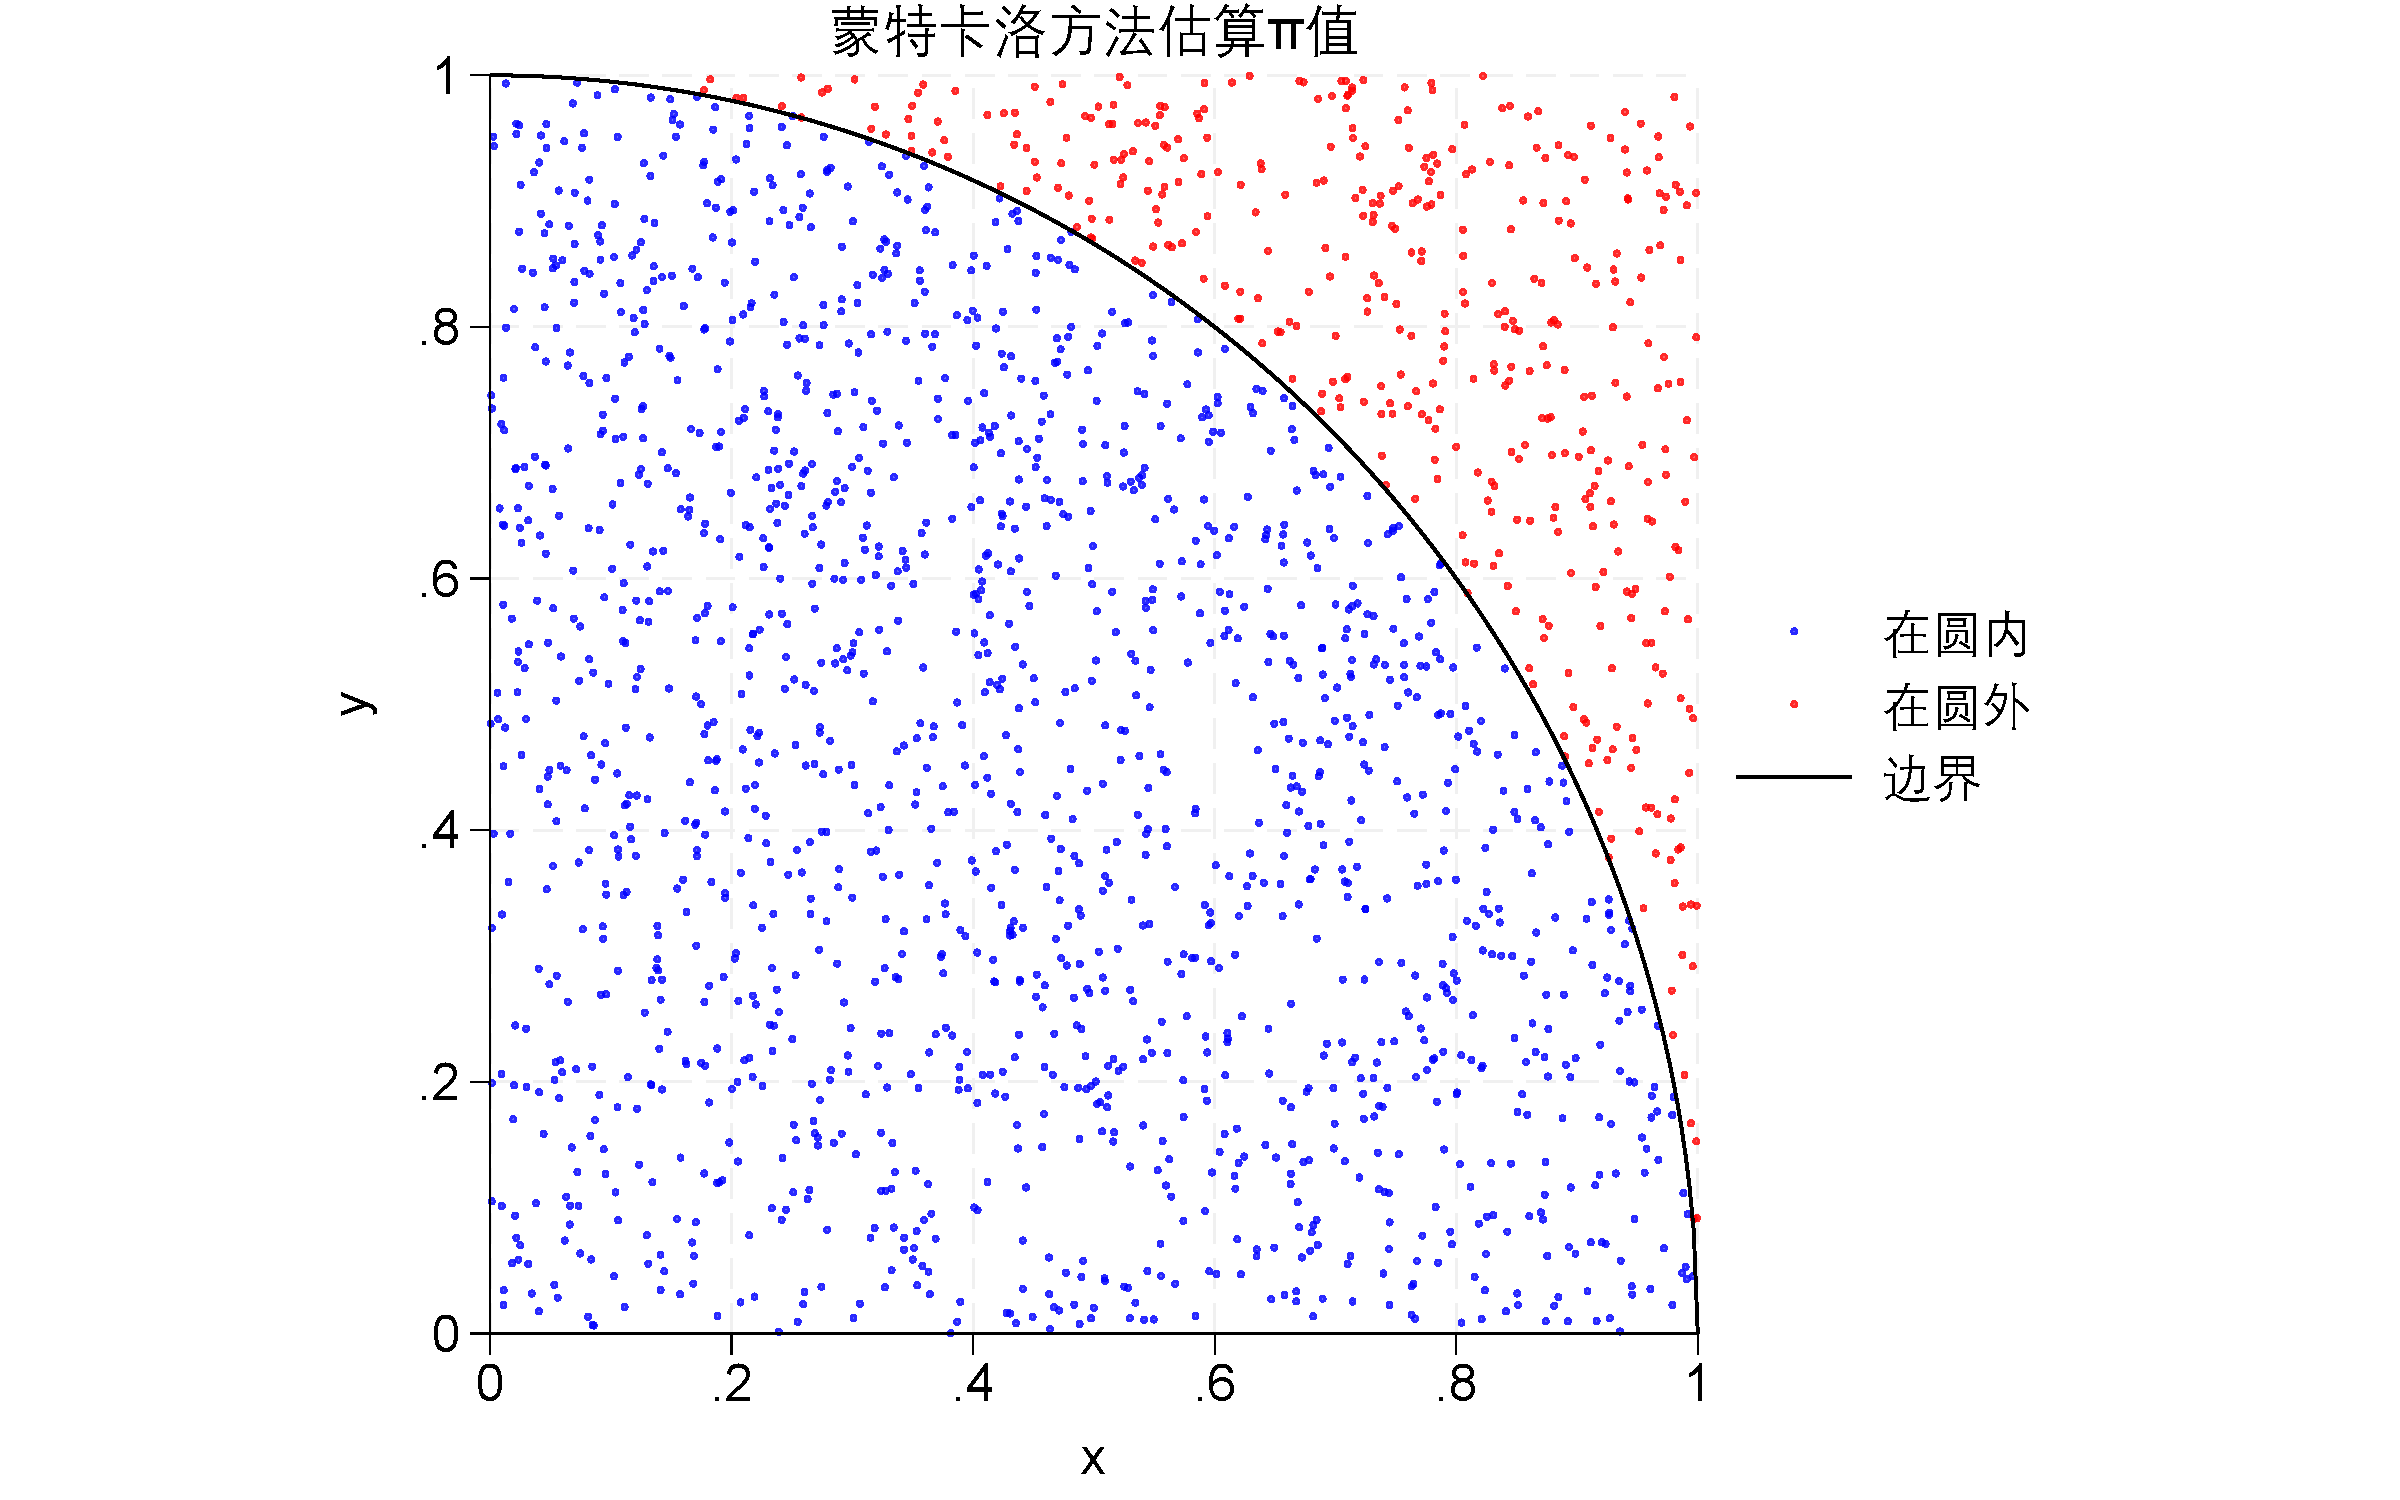
\includegraphics[width=0.8\textwidth]{image/circle_pi.pdf}
	\end{center}
\end{tcolorbox}

\begin{tcolorbox}[title=在 Stata 中运用模拟法验证大样本假定, colback=white, colframe=black, colbacktitle=white, coltitle=black,fonttitle=\bfseries]
	\begin{lstlisting}[xleftmargin=2em,
		basicstyle=\ttfamily\small\color{black},
		keywordstyle=\color{black},
		commentstyle=\color{black},
		stringstyle=\color{black},
		identifierstyle=\color{black},
		numberstyle=\color{black},
		showstringspaces=false,
		morekeywords={clear, set, seed, net, install, mc_ols_sim, from, replace, use, collapse, list, twoway, histogram, kdensity, line, title, legend, yline, xline, aspectratio, plotregion, graphregion, save, color}]
clear all // 清除内存中所有数据和程序
set seed 12345 // 设置随机数种子,确保结果可重现

// 安装ado文件
net install mc_ols_sim, from(https://gitee.com/yuanjingyang2/mc_ols_sim/raw/master) replace
// 运行蒙特卡洛模拟 - 不同样本容量
mc_ols_sim, n(10 30 50 100 200 500 700 1000) dist(poisson) reps(1000) beta0(1) beta1(0.2)
// 运行1000次模拟,样本量包含10-1000,其中的分布选项对应泊松

// 定义语法,n为样本量列表,dist为分布类型——默认为uniform,其中可选分布选项:uniform(均匀) normal(正态) binomial(二项) poisson(泊松) exponential(指数) cauchy(柯西) chi2(卡方),reps为模拟次数默认1000,beta0和beta1为回归系数默认值1和2。

// 分析结果 - 大数定律验证
use results.dta, clear // 调用存储的结果数据
collapse (mean) b0 b1, by(n) // 按样本量分组计算估计量均值
list // 显示结果

twoway (line b0 n, lcolor(blue) lpattern(solid)) ///  绘制截距估计均值线
       (line b1 n, lcolor(red) lpattern(solid)), ///  绘制斜率估计均值线
       yline(1 2, lpattern(dash) lcolor(black%20)) ///  添加真值参考线
       legend(order(1 "截距估计均值" 2 "斜率估计均值") pos(6) cols(3)) ///  添加图例
       title("大数定律:估计量收敛到真值") // 添加标题

// 分析结果 - 中心极限定理验证
use results.dta, clear // 重新调用数据

twoway ///
    (histogram b1 if n==10, width(0.1) percent color(blue%10) yaxis(1)) ///  n=10直方图
    (kdensity b1 if n==10, lcolor(blue) lwidth(medthick) yaxis(2)) ///  n=10核密度
    (histogram b1 if n==100, width(0.1) percent color(purple%10) yaxis(1)) ///  n=100直方图
    (kdensity b1 if n==100, lcolor(purple) lwidth(medthick) yaxis(2)) ///  n=100核密度
    (histogram b1 if n==1000, width(0.1) percent color(red%10) yaxis(1)) ///  n=1000直方图
    (kdensity b1 if n==1000, lcolor(red) lwidth(medthick) yaxis(2)), ///  n=1000核密度
    legend(order(4 "n=10" 5 "n=100" 6 "n=1000") pos(6) cols(3)) ///
    title("不同样本量下斜率估计量分布的对比") ///
    xtitle("斜率估计值") ///
    ytitle("百分比", axis(1)) ///
    ytitle("密度", axis(2))
	\end{lstlisting}
\end{tcolorbox}

\begin{tcolorbox}[title=在 Stata 中运用模拟法验证大样本假定, colback=white, colframe=black, colbacktitle=white, coltitle=black,fonttitle=\bfseries]

	\begin{center}
	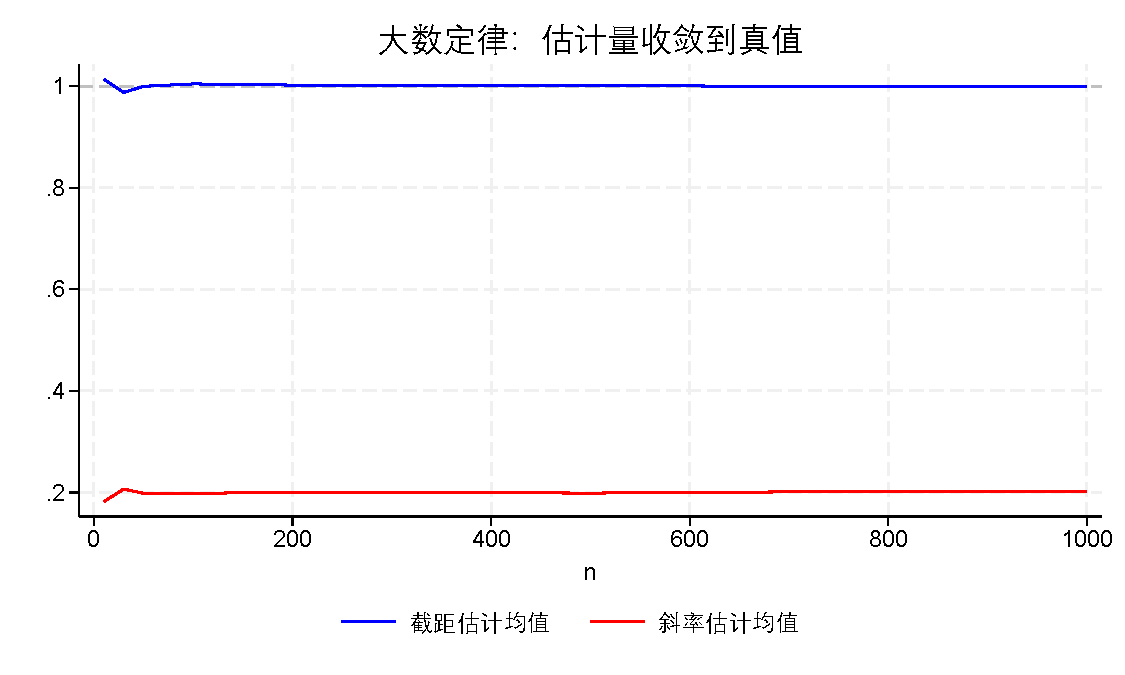
\includegraphics[width=0.8\textwidth]{image/large_numbers.pdf}
	\end{center}
	\begin{center}
	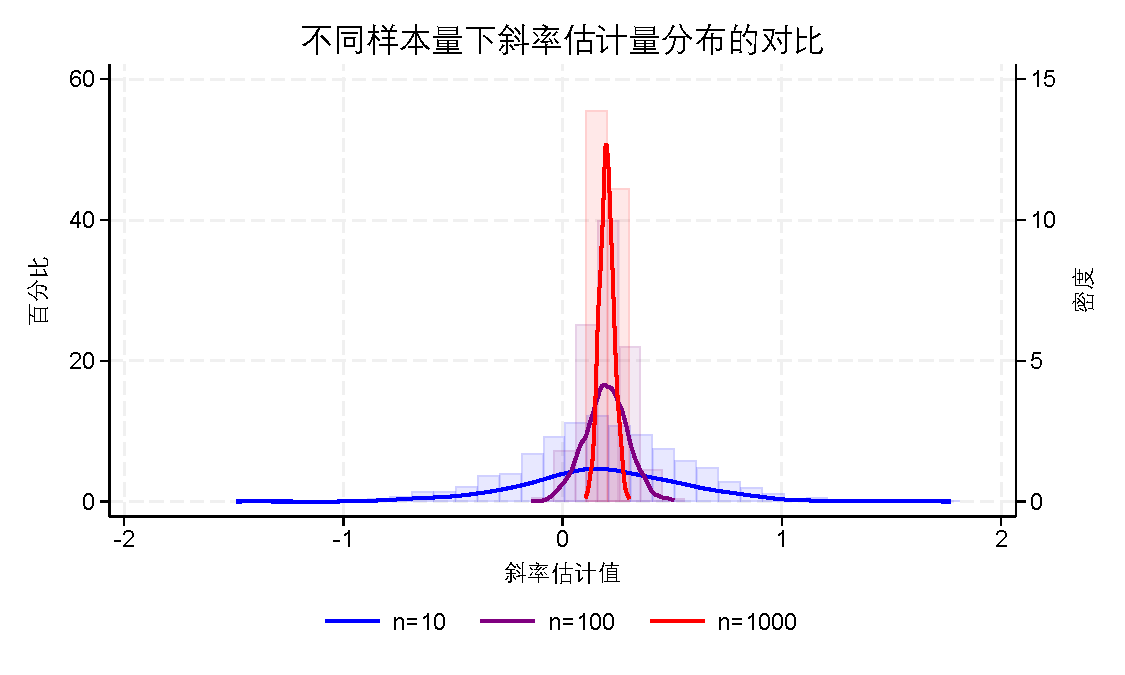
\includegraphics[width=0.8\textwidth]{image/central_limit.pdf}
	\end{center}
\end{tcolorbox}

\paragraph*{异方差问题}

在大多数计量经济学模型中,一个核心的假设是误差项的方差为常数,即满足同方差性(homoskedasticity)。然而,在许多现实世界的场景中,这一假设往往被违反,即误差项的方差会随着解释变量的变化而变化,此现象称为异方差性(heteroskedasticity)。异方差问题的存在导致普通最小二乘(OLS)估计量虽然仍是无偏且一致的,但不再是有效的(即不再具有最小方差),其计算的标准误会产生偏误,进而使基于这些标准误的假设检验(如t检验、F检验和Wald检验)以及置信区间失效,导致错误的统计推断。

我们通过一个模拟数据来展示异方差问题:

\begin{tcolorbox}[title=在 Stata 中展示异方差问题, colback=white, colframe=black, colbacktitle=white, coltitle=black,fonttitle=\bfseries]
	\begin{lstlisting}[xleftmargin=2em,
		basicstyle=\ttfamily\small\color{black},
		keywordstyle=\color{black},
		commentstyle=\color{black},
		stringstyle=\color{black},
		identifierstyle=\color{black},
		numberstyle=\color{black},
		showstringspaces=false,
		morekeywords={clear, set, seed, net, install, mc_ols_sim, from, replace, use, collapse, list, twoway, histogram, kdensity, line, title, legend, yline, xline, aspectratio, plotregion, graphregion, save, color}]
clear
set obs 500
set seed 12345

gen x = runiform(0, 10)
gen sigma = 0.5 + 0.5*x
gen u = rnormal(0, sigma)
gen y = 2 + 1.5*x + u

reg y x
predict resid, residuals
predict yhat, xb

twoway (scatter y x) (lfit y x), ///
    title("原始数据与拟合回归线") ///
    ytitle("y") ///
    xtitle("x") ///
    legend(order(1 "数据点" 2 "拟合线") cols(1) position(6)) ///
    name(graph1, replace)

twoway (scatter resid x) (lowess resid x, lcolor(red)), ///
    title("异方差诊断图") ///
    ytitle("残差") ///
    xtitle("x") ///
    legend(order(1 "残差点" 2 "局部加权回归线") cols(1) position(6)) ///
    name(graph2, replace)

graph combine graph1 graph2, cols(2) title("分析结果")
	\end{lstlisting}
	\vspace{2em}
	\begin{center}
	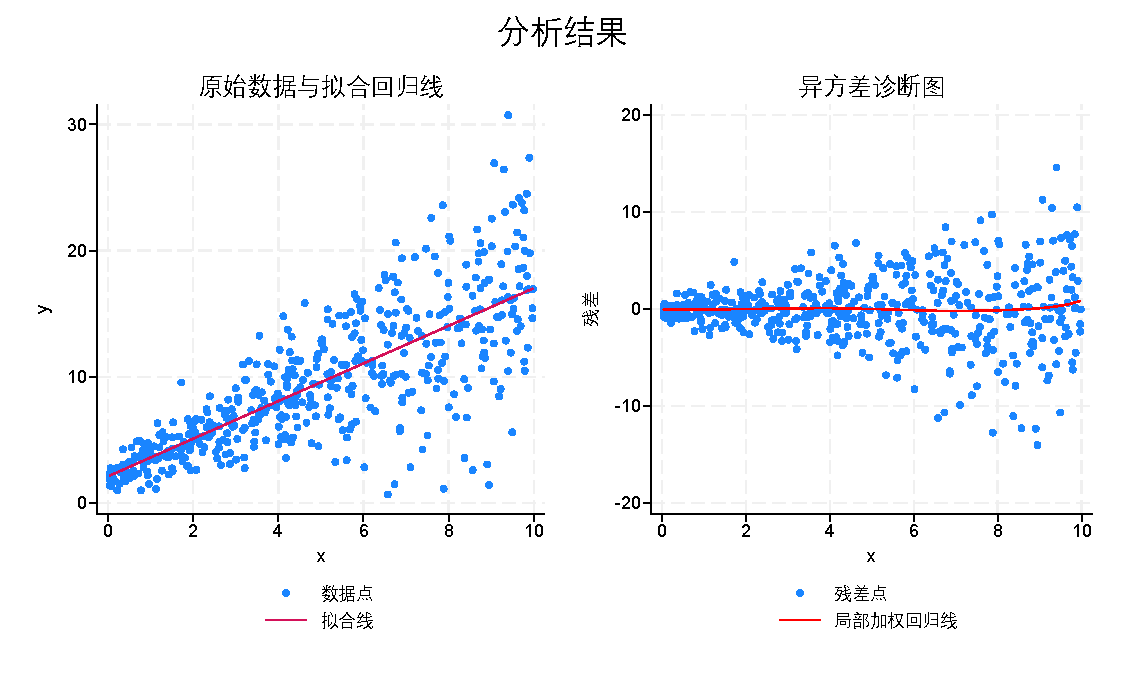
\includegraphics[width=0.8\textwidth]{image/heteroskedasticity.pdf}
	\end{center}
\end{tcolorbox}

\textbf{1. 异方差稳健标准误(Heteroskedasticity-Robust Standard Errors)}

在满足条件期望为零($\mathbb{E}[\epsilon_i|\bm{X}_i]=0$)但允许 $\mathrm{Var}(\epsilon_i|\bm{X}_i)=\sigma_i^2$ 随 $i$ 变化的情形下,OLS 点估计 $\hat{\bm{\beta}}=(\bm{X}'\bm{X})^{-1}\bm{X}'\bm{Y}$ 仍是一致的,但传统同方差方差公式 $s^2(\bm{X}'\bm{X})^{-1}$ 不再一致。White(1980)提出的异方差稳健(Eicker–Huber–White)协方差估计量在不预设异方差具体形式的前提下,给出对 $\mathrm{Var}(\hat{\bm{\beta}}|\bm{X})$ 的一致估计,从而保证大样本下的 $t$ 检验、Wald 检验与置信区间有效。

\textbf{数学推导}
在异方差下,OLS估计量的条件真方差为:

\begin{equation}
	\mathrm{Var}(\hat{\bm{\beta}}|\bm{X}) = (\bm{X}'\bm{X})^{-1}\bm{X}'\bm{\Omega}\bm{X}(\bm{X}'\bm{X})^{-1}
\end{equation}

其中,$\bm{\Omega} = \mathrm{diag}(\sigma_1^2,\dots,\sigma_n^2)$ 是误差项 $\bm{\epsilon}$ 的方差-协方差矩阵,它是一个对角矩阵,其对角线元素为各个观测点误差项的异方差。

White(1980)提出用 OLS 残差的平方 $\hat{e}_i^{\,2}$ 作为对未知异方差 $\sigma_i^2$ 的一致估计量。因此,对于中间的“夹心”部分 $\bm{X}'\bm{\Omega}\bm{X}$,我们可以用其样本类似物进行一致估计:

\begin{equation}
	\widehat{\bm{S}} = \sum_{i=1}^n \hat e_i^{\,2}\,\bm{X}_i\bm{X}_i'
\end{equation}

其中 $\bm{X}_i$ 是第 $i$ 个观测值的解释变量行向量(表示为列向量),$\hat e_i$ 是 OLS 残差。
将此样本类似物代入真方差公式,即可得到异方差稳健协方差的估计量:

\begin{equation}
	\begin{split}
		\widehat{\mathrm{Var}}_{\mathrm{robust}}(\hat{\bm{\beta}})
		&= (\bm{X}'\bm{X})^{-1}\left(\sum_{i=1}^n \hat e_i^{\,2}\,\bm{X}_i\bm{X}_i'\right)(\bm{X}'\bm{X})^{-1} \\
		&= (\bm{X}'\bm{X})^{-1}\bm{X}'\,\mathrm{diag}(\hat e_1^{\,2},\dots,\hat e_n^{\,2})\,\bm{X}\,(\bm{X}'\bm{X})^{-1}
	\end{split}
\end{equation}

这个结构常被形象地称作“三明治(sandwich)”形式:两侧的“面包”是 $(\bm{X}'\bm{X})^{-1}$,中间的“夹心”是 $\bm{X}'\,\mathrm{diag}(\hat e_1^{\,2},\dots,\hat e_n^{\,2})\,\bm{X}$。

\textbf{统计推断与报告}
令 $\widehat{\mathrm{Var}}_{\mathrm{robust}}(\hat{\bm{\beta}})=\hat{\bm{V}}$,则第 $k$ 个系数的稳健标准误为 $\mathrm{se}_k=\sqrt{\hat V_{kk}}$。
\begin{itemize}
  \item \textbf{不改变点估计}:异方差稳健标准误不改变原始OLS系数估计值,仅修正其标准误。
  \item \textbf{t 检验}:$t_k=\hat\beta_k/\mathrm{se}_k$。在大样本下,可用标准正态分布进行近似检验。
  \item \textbf{置信区间}:$\hat\beta_k \pm z_{1-\alpha/2}\,\mathrm{se}_k$(或在有限样本中用更保守的临界值)。
\end{itemize}
White 稳健标准误以简洁的三明治结构在不改变 OLS 点估计的前提下,为异方差环境下的大样本推断提供一致的标准误与检验基础,已成为应用计量经济学的“默认选项”之一。

在 Stata 中,可以通过 \texttt{robust} 选项实现:

\begin{tcolorbox}[title=在 Stata 中解决异方差问题, colback=white, colframe=black, colbacktitle=white, coltitle=black,fonttitle=\bfseries]
	\begin{lstlisting}[xleftmargin=2em,
		basicstyle=\ttfamily\small\color{black},
		keywordstyle=\color{black},
		commentstyle=\color{black},
		stringstyle=\color{black},
		identifierstyle=\color{black},
		numberstyle=\color{black},
		showstringspaces=false,
		morekeywords={clear, set, seed, net, install, mc_ols_sim, from, replace, use, collapse, list, twoway, histogram, kdensity, line, title, legend, yline, xline, aspectratio, plotregion, graphregion, save, color}]
clear
set obs 500
set seed 12345

gen x = runiform(0, 10)
gen sigma = 0.5 + 0.5*x
gen u = rnormal(0, sigma)
gen y = 2 + 1.5*x + u

reg y x
reg y x, robust
di "显然的,加入robust选项后x的标准误增加,t减小,即此时如果仍然显著,则更加稳健。"
	\end{lstlisting}
	\vspace{-1em}
	\begin{Verbatim}[commandchars=\\\{\},xleftmargin=2em]
. reg y x
      Source |       SS           df       MS      Number of obs   =       500
-------------+----------------------------------   F(1, 498)       =    772.97
       Model |  9384.67049         1  9384.67049   Prob > F        =    0.0000
    Residual |  6046.21789       498  12.1409998   R-squared       =    0.6082
-------------+----------------------------------   Adj R-squared   =    0.6074
       Total |  15430.8884       499   30.923624   Root MSE        =    3.4844

------------------------------------------------------------------------------
           y | Coefficient  Std. err.      t    P>|t|     [95% conf. interval]
-------------+----------------------------------------------------------------
           x |   1.490595   .0536139    27.80   0.000     1.385258    1.595933
       _cons |   2.120809   .3037144     6.98   0.000     1.524089    2.717528
------------------------------------------------------------------------------
. reg y x, robust
Linear regression                               Number of obs     =        500
                                                F(1, 498)         =     636.51
                                                Prob > F          =     0.0000
                                                R-squared         =     0.6082
                                                Root MSE          =     3.4844

------------------------------------------------------------------------------
             |               Robust
           y | Coefficient  std. err.      t    P>|t|     [95% conf. interval]
-------------+----------------------------------------------------------------
           x |   1.490595   .0590822    25.23   0.000     1.374514    1.606676
       _cons |   2.120809   .1961559    10.81   0.000     1.735414    2.506204
------------------------------------------------------------------------------
显然的,加入robust选项后x的标准误增加,t减小,即此时如果仍然显著,则更加稳健。
	\end{Verbatim}
\end{tcolorbox}

\textbf{2. 广义最小二乘法(Generalized Least Squares, GLS)}

广义最小二乘法(GLS)是处理异方差和(或)自相关问题的一种有效方法。其核心思想是:当误差项的方差—协方差矩阵不满足球形假设(即误差项既非同方差也非不相关)时,通过对模型进行线性变换,使得扰动项在转换后的模型中重新满足同方差和不相关性,进而利用OLS方法对转换后的模型进行估计。GLS不仅适用于异方差问题,也可推广至处理序列相关与更一般的相关结构。

\textbf{理论基础}

考虑线性回归模型:

\begin{equation}
	\bm{Y} = \bm{X}\bm{\beta} + \bm{\epsilon}
\end{equation}

其中 $\mathbb{E}(\bm{\epsilon}|\bm{X}) = \bm{0}$,但 $\mathrm{Var}(\bm{\epsilon}|\bm{X}) = \bm{\Omega}$,且 $\bm{\Omega} \neq \sigma^2 \bm{I}_n$。
GLS通过构造一个可逆的变换矩阵 $\bm{P}$,使得转换后的误差项 $\bm{\epsilon}^* = \bm{P}\bm{\epsilon}$ 满足球形扰动项假设,即 $\mathrm{Var}(\bm{\epsilon}^*|\bm{X}) = \sigma^2 \bm{I}_n$。

\textbf{数学推导}

我们寻找一个变换矩阵 $\bm{P}$,使得 $\mathrm{Var}(\bm{P}\bm{\epsilon}|\bm{X}) = \bm{P}\mathrm{Var}(\bm{\epsilon}|\bm{X})\bm{P}' = \bm{P}\bm{\Omega}\bm{P}' = \sigma^2 \bm{I}_n$。
若 $\bm{\Omega}$ 是一个正定矩阵,则其平方根逆矩阵 $\bm{P} = \bm{\Omega}^{-1/2}$ 存在。令 $\sigma^2=1$ 不失一般性(因为最终 $\sigma^2$ 会被估计并纳入方差),则选择 $\bm{P} = \bm{\Omega}^{-1/2}$,可以使:

\begin{equation}
	\begin{split}
		\mathrm{Var}(\bm{P}\bm{\epsilon}|\bm{X}) &= \bm{\Omega}^{-1/2} \bm{\Omega} (\bm{\Omega}^{-1/2})' \\
		&= \bm{\Omega}^{-1/2} \bm{\Omega} \bm{\Omega}^{-1/2} \\
		&= \bm{I}_n
	\end{split}
\end{equation}

对原始模型 $\bm{Y} = \bm{X}\bm{\beta} + \bm{\epsilon}$ 两边左乘 $\bm{P}$,得到转换后的模型:

\begin{equation}
	\bm{P}\bm{Y} = \bm{P}\bm{X}\bm{\beta} + \bm{P}\bm{\epsilon}
	\quad \text{或写为} \quad \bm{Y}^* = \bm{X}^*\bm{\beta} + \bm{\epsilon}^*
\end{equation}

其中 $\bm{Y}^*=\bm{P}\bm{Y}$,$\bm{X}^*=\bm{P}\bm{X}$,$\bm{\epsilon}^*=\bm{P}\bm{\epsilon}$。
此时,转换后的误差项 $\bm{\epsilon}^*$ 满足同方差和不相关性假设,因此可以对转换后的模型应用OLS,得到的估计量即为GLS估计量:

\begin{equation}
	\begin{split}
		\hat{\bm{\beta}}_{\mathrm{GLS}} &= ((\bm{P}\bm{X})'(\bm{P}\bm{X}))^{-1}(\bm{P}\bm{X})'(\bm{P}\bm{Y}) \\
		&= (\bm{X}'\bm{P}'\bm{P}\bm{X})^{-1}\bm{X}'\bm{P}'\bm{P}\bm{Y} \\
		&= (\bm{X}'\bm{\Omega}^{-1/2}\bm{\Omega}^{-1/2}\bm{X})^{-1}\bm{X}'\bm{\Omega}^{-1/2}\bm{\Omega}^{-1/2}\bm{Y} \\
		&= (\bm{X}'\bm{\Omega}^{-1}\bm{X})^{-1}\bm{X}'\bm{\Omega}^{-1}\bm{Y}
	\end{split}
\end{equation}

根据Gauss-Markov定理,$\hat{\bm{\beta}}_{\mathrm{GLS}}$ 是线性、无偏且有效的(BLUE)。

当 $\bm{\Omega}$ 未知时,需要通过某种方式对其进行估计,得到 $\hat{\bm{\Omega}}$。将 $\hat{\bm{\Omega}}$ 代替 $\bm{\Omega}$ 即可得到可行广义最小二乘(Feasible GLS, FGLS)估计量:

\begin{equation}
	\hat{\bm{\beta}}_{\mathrm{FGLS}} = (\bm{X}'\hat{\bm{\Omega}}^{-1}\bm{X})^{-1}\bm{X}'\hat{\bm{\Omega}}^{-1}\bm{Y}
\end{equation}

在正则条件下,FGLS具有与GLS相同的渐近性质,即渐近有效。

\textbf{与加权最小二乘(WLS)的关系}

当 $\bm{\Omega}$ 是一个对角矩阵(即仅存在异方差,无自相关)时,GLS估计量退化为加权最小二乘(Weighted Least Squares, WLS)估计量。此时,$\bm{\Omega}^{-1}$ 也是对角矩阵,其对角线元素为各观测值方差的倒数 $1/\sigma_i^2$,扮演了权重矩阵的角色。

\textbf{注意事项}
\begin{itemize}
\item GLS和FGLS要求对误差项的方差—协方差结构有正确的设定或准确的估计。若对 $\bm{\Omega}$ 的设定或估计有误,FGLS可能反而不如OLS(因社科数据通常难以完全掌握DGP,故很少使用)。
\item 在小样本情况下,由于 $\hat{\bm{\Omega}}$ 的估计误差,FGLS的表现不一定优于OLS。在大样本下,FGLS通常能显著提高估计的精度和效率。
\item 在实证研究中,若采用FGLS,应在转换并回归后重新检验异方差是否已被消除。
\end{itemize}

\textbf{3. 聚类稳健标准误(Cluster-Robust Standard Errors)}

在许多实证研究中,数据往往具有固有的群组(或集群)结构,例如来自同一学校的学生、同一公司内的员工,或同一地理区域的住户等。在这种情况下,同一群组内的观测值通常会受到共同的、未被模型捕获的因素影响,导致其误差项之间存在相关性。传统的普通最小二乘(OLS)标准误假设误差项是独立同分布的(i.i.d.),即使修正了异方差(如White标准误),也无法处理群组内部的相关性。忽略这种群组内的相关性会导致标准误被系统性低估,从而夸大估计结果的统计显著性,造成错误的推断。

聚类稳健标准误(Cluster-Robust Standard Errors, CRSE)旨在纠正这一问题。其核心思想是允许同一群组内的误差项存在任意形式的相关性(包括异方差和自相关),但假定不同群组间的误差项是相互独立的。在聚类稳健标准误下,OLS估计量 $\hat{\pmb{\beta}}^{\text{OLS}}$ 依然是无偏且一致的,但其标准误的计算方式需要调整。

\textbf{数学推导}

我们从OLS估计量方差的普遍形式出发:
\begin{equation}
	\operatorname{Var} \left( \hat{\pmb{\beta}}^{\text{OLS}} \right) = (\pmb{X}^{\prime}\pmb{X})^{-1} \pmb{X}^{\prime} E[\pmb{e}\pmb{e}^{\prime}] \pmb{X} (\pmb{X}^{\prime}\pmb{X})^{-1}
\end{equation}
其中,$\pmb{\Omega} = E[\pmb{e}\pmb{e}^{\prime}]$ 是误差项 $\pmb{e}$ 的方差-协方差矩阵。

在数据存在群组结构的情况下,假设总共有 $G$ 个群组,每个群组 $g$ 包含 $T_g$ 个观测值。我们将总的误差向量 $\pmb{e}$ 和解释变量矩阵 $\pmb{X}$ 相应地按群组进行划分:
\begin{equation}
	\pmb{e} = \begin{pmatrix} \pmb{e}_1 \\ \pmb{e}_2 \\ \vdots \\ \pmb{e}_G \end{pmatrix}, \quad \pmb{X} = \begin{pmatrix} \pmb{X}_1 \\ \pmb{X}_2 \\ \vdots \\ \pmb{X}_G \end{pmatrix}
\end{equation}
其中 $\pmb{e}_g$ 是第 $g$ 个群组的误差向量($T_g \times 1$),$\pmb{X}_g$ 是第 $g$ 个群组的解释变量矩阵($T_g \times K$,$K$ 为解释变量数量)。

聚类稳健标准误的核心假设是:群组间的误差项是相互独立的,而群组内的误差项可以任意相关。这意味着误差项的方差-协方差矩阵 $\pmb{\Omega}$ 呈现出块对角(block-diagonal)结构:
\begin{equation}
	\begin{split}
		\pmb{\Omega}_{\text{cluster}} = E[\pmb{e}\pmb{e}^{\prime}] \\
		&= \begin{pmatrix} 
		E[\pmb{e}_1\pmb{e}_1^{\prime}] & \pmb{0} & \cdots & \pmb{0} \\
		\pmb{0} & E[\pmb{e}_2\pmb{e}_2^{\prime}] & \cdots & \pmb{0} \\
		\vdots & \vdots & \ddots & \vdots \\
		\pmb{0} & \pmb{0} & \cdots & E[\pmb{e}_G\pmb{e}_G^{\prime}]
		\end{pmatrix} \\
		&= \operatorname{diag}(\pmb{\Omega}_1, \pmb{\Omega}_2, \dots, \pmb{\Omega}_G)
	\end{split}
\end{equation}
其中 $\pmb{\Omega}_g = E[\pmb{e}_g\pmb{e}_g^{\prime}]$ 是第 $g$ 个群组的误差项方差-协方差矩阵,它允许非对角线元素非零,即群组内部存在相关性。

将此块对角矩阵代入OLS估计量的方差公式:
\begin{equation}
	\begin{split}
		\operatorname{Var} \left( \hat{\pmb{\beta}}^{\text{OLS}} \right) &= (\pmb{X}^{\prime}\pmb{X})^{-1} \pmb{X}^{\prime} \pmb{\Omega}_{\text{cluster}} \pmb{X} (\pmb{X}^{\prime}\pmb{X})^{-1} \\
		&= (\pmb{X}^{\prime}\pmb{X})^{-1} \left( \sum_{g=1}^{G} \pmb{X}_g^{\prime} \pmb{\Omega}_g \pmb{X}_g \right) (\pmb{X}^{\prime}\pmb{X})^{-1}
	\end{split}
\end{equation}
为了估计这个方差,我们用样本残差 $\hat{\pmb{e}}_g = \pmb{Y}_g - \pmb{X}_g \hat{\pmb{\beta}}^{\text{OLS}}$ 来近似 $\pmb{e}_g$,并用样本协方差 $\hat{\pmb{e}}_g \hat{\pmb{e}}_g^{\prime}$ 来近似真实的 $\pmb{\Omega}_g = E[\pmb{e}_g\pmb{e}_g^{\prime}]$。因此,聚类稳健标准误的估计公式为:
\begin{equation}
	\widehat{\operatorname{Var}} \left( \hat{\pmb{\beta}}_{\text{cluster}}^{\text{OLS}} \right) = (\pmb{X}^{\prime}\pmb{X})^{-1} \left[ \sum_{g=1}^{G} \pmb{X}_{g}^{\prime} \hat{\pmb{e}}_{g} \hat{\pmb{e}}_{g}^{\prime} \pmb{X}_{g} \right] (\pmb{X}^{\prime}\pmb{X})^{-1}
\end{equation}
在实际应用中,通常还会加入小样本调整项,例如乘以 $\frac{G}{G-1}$ 或 $\frac{N-1}{N-K} \frac{G}{G-1}$,其中 $N$ 是总观测数,$K$ 是解释变量的数量。

\textbf{使用须知}

聚类稳健标准误允许误差项在群组内任意相关和异方差,但在群组间保持独立。它在群组数量 $G$ 足够大时(通常认为至少20-30个群组)是OLS估计量方差的一致估计。当群组数量过少时,聚类稳健标准误可能表现不佳。因此,在选择聚类标准误时,研究者需要仔细考虑群组的定义以及群组的数量。

在 Stata 中,可以使用 \texttt{cluster} 选项实现,例如按组变量 \texttt{groupid} 聚类:

\begin{tcolorbox}[title=在 Stata 中实现加权-聚类稳健标准误, colback=white, colframe=black, colbacktitle=white, coltitle=black,fonttitle=\bfseries]
	\begin{lstlisting}[xleftmargin=2em,
		basicstyle=\ttfamily\small\color{black},
		keywordstyle=\color{black},
		commentstyle=\color{black},
		stringstyle=\color{black},
		identifierstyle=\color{black},
		numberstyle=\color{black},
		showstringspaces=false,
		morekeywords={clear, set, seed, net, install, mc_ols_sim, from, replace, use, collapse, list, twoway, histogram, kdensity, line, title, legend, yline, xline, aspectratio, plotregion, graphregion, save, color, table}]
// 生成同时具有异方差和聚类相关性的数据
clear all
qui set obs 1500

// 生成聚类结构
gen group_id = ceil(_n/5)  // 300个组,每组5个观测
gen x1 = rnormal(0,1)
gen x2 = rnormal(0,1)
gen z = runiform(0,1)

// 生成异方差结构
gen sigma = exp(0.3*z)  // 异方差结构
gen group_fe = rnormal(0,0.3)  // 组层面固定效应

// 扩展组固定效应到所有观测
qui bysort group_id: replace group_fe = group_fe[1]

// 生成误差项
gen e = rnormal(0,sigma)
gen y = 1 + 2*x1 + 1.5*x2 + group_fe + e  // 真实模型

// 第一步:普通OLS
qui reg y x1 x2
estimates store ols

// 第二步:估计异方差结构
qui predict resid, residuals  // 获取残差
gen log_resid2 = log(resid^2)  // 残差平方的对数
qui reg log_resid2 z  // 回归估计方差函数
qui predict fitted_log_resid2  // 预测log(σ²)
gen estimated_sigma = sqrt(exp(fitted_log_resid2))  // 估计σ
gen weights = 1/(estimated_sigma^2)  // 计算权重

// 第三步:加权最小二乘
qui reg y x1 x2 [aweight=weights]
estimates store wls

// 第四步:聚类稳健标准误
qui reg y x1 x2, cluster(group_id)
estimates store clustered_se

// 第五步:同时使用权重和聚类稳健标准误
qui reg y x1 x2 [aweight=weights], cluster(group_id)
estimates store wls_clustered

// 比较所有结果
estimates table ols wls clustered_se wls_clustered, b(%9.4f) se stats(N r2)
\end{lstlisting}
\end{tcolorbox}

\begin{tcolorbox}[title=在 Stata 中实现加权-聚类稳健标准误, colback=white, colframe=black, colbacktitle=white, coltitle=black,fonttitle=\bfseries]

	\begin{Verbatim}[commandchars=\\\{\},xleftmargin=2em]
. estimates table ols wls clustered_se wls_clustered, b(%9.4f) se stats(N r2)
--------------------------------------------------------------
    Variable |    ols         wls      cluster~e   wls_clu~d  
-------------+------------------------------------------------
          x1 |    1.9715      1.9738      1.9715      1.9738  
             |    0.0322      0.0320      0.0313      0.0310  
          x2 |    1.4718      1.4713      1.4718      1.4713  
             |    0.0320      0.0318      0.0317      0.0314  
       _cons |    0.9053      0.9058      0.9053      0.9058  
             |    0.0317      0.0316      0.0356      0.0354  
-------------+------------------------------------------------
           N |      1500        1500        1500        1500  
          r2 |    0.7985      0.8005      0.7985      0.8005  
--------------------------------------------------------------
                                                  Legend: b/se

	\end{Verbatim}

\end{tcolorbox}

\section{非OLS回归与时空计量经济学}

当古典线性回归模型的假定(特别是关于误差项的假定)不再成立时,我们需要转向更广义的回归方法。本节将介绍当因变量为离散或受限类型,以及当数据包含时间或空间维度时所采用的专门模型。这些模型扩展了统计推断的边界,使其能够处理更复杂的社会科学问题。

\subsection{离散与受限因变量}

在许多研究中,因变量并非连续变量,而是表现为类别、计数或在某个范围内受限的形式。例如,投票选择(支持/反对)、事故发生次数或家庭耐用品支出(不能为负)。在这种情况下,使用普通最小二乘法(OLS)是不恰当的,因为它可能产生无意义的预测(如概率大于1或小于0),并且其线性假定本身也存在问题。

\paragraph*{线性概率模型(LPM)的局限}
对于二元因变量(取值为0或1),最简单的方法是使用OLS,这被称为\textbf{线性概率模型(Linear Probability Model, LPM)}。尽管LPM的系数易于解释(表示自变量变化一单位,因变量取1的概率变化多少),但它存在严重缺陷:
\begin{enumerate}
    \item \textbf{预测概率越界}:LPM的拟合值(即预测概率)可能超出[0, 1]的合理范围。
    \item \textbf{非线性关系}:自变量对概率的边际效应通常不是恒定的,而LPM假设其为线性。
    \item \textbf{异方差性}:当因变量为0-1分布时,误差项的方差依赖于解释变量的值,即
    \[
    \text{Var}(\varepsilon_i | \mathbf{X}) = p_i(1-p_i)
    \]
    这违反了同方差假定。
\end{enumerate}

为了克服这些问题,我们需要使用专门为离散或受限因变量设计的非线性模型。

\paragraph*{二元选择模型:Logit与Probit}
当因变量是二元选择时(如是否就业、是否投票),通常使用\textbf{Logit模型}和\textbf{Probit模型}。这两种模型都通过一个非线性的累积分布函数(Cumulative Distribution Function, CDF)将自变量的线性组合映射到(0, 1)区间,从而保证预测概率的有效性。

\textbf{Logit模型}假设潜在误差项服从Logistic分布(Logistic Distribution)。其概率表达式为:
\begin{equation}
P(Y_i=1 | \mathbf{X}_i) = \Lambda(\mathbf{X}_i'\boldsymbol{\beta}) = \frac{\exp(\mathbf{X}_i'\boldsymbol{\beta})}{1 + \exp(\mathbf{X}_i'\boldsymbol{\beta})}
\end{equation}
其中 $\Lambda(\cdot)$ 是Logistic分布的CDF。Logit模型的系数可以解释为对数几率(log-odds ratio)的变化。

\textbf{Probit模型}假设潜在误差项服从标准正态分布。其概率表达式为:
\begin{equation}
P(Y_i=1 | \mathbf{X}_i) = \Phi(\mathbf{X}_i'\boldsymbol{\beta}) = \int_{-\infty}^{\mathbf{X}_i'\boldsymbol{\beta}} \frac{1}{\sqrt{2\pi}} \exp\left(-\frac{z^2}{2}\right) dz
\end{equation}
其中 $\Phi(\cdot)$ 是标准正态CDF。

由于模型的非线性,Logit和Probit模型的系数本身并不直接等于边际效应。我们需要计算\textbf{平均边际效应(Average Marginal Effects, AME)}来解释自变量对概率的影响。

\begin{figure}[htbp]
	\centering
	\fbox{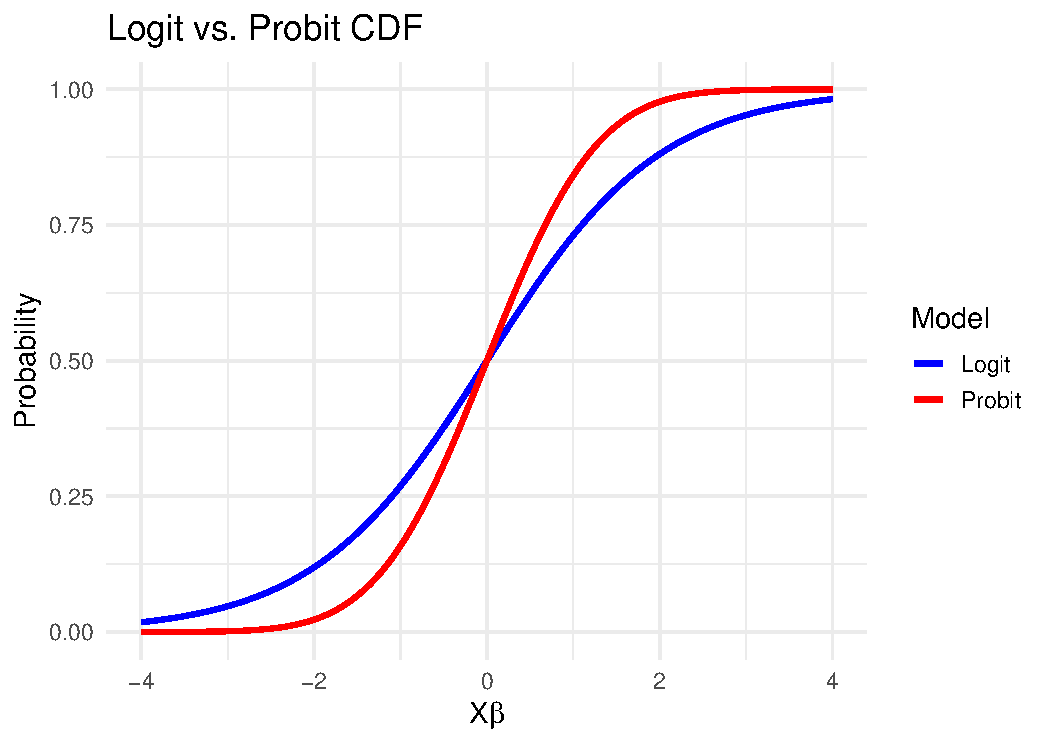
\includegraphics[width=0.7\textwidth]{image/logit_probit_cdf.pdf}}
	\caption[两个分布的CDF]{两个分布的CDF}
	\label{fig:logit_probit_cdf}
\end{figure}

\begin{tcolorbox}[title=在 Stata 中估计 Probit 模型并计算边际效应, colback=white, colframe=black, colbacktitle=white, coltitle=black,fonttitle=\bfseries]
\begin{lstlisting}[xleftmargin=2em, commentstyle=\color{black}]
quietly sysuse auto, clear

*线性模型
qui regress foreign mpg weight
est store lpm

*Logit 模型
qui logit foreign mpg weight
est store logit_model
margins, dydx(*) // 计算平均边际效应

*Probit 模型
qui probit foreign mpg weight
est store probit_model
margins, dydx(*) // 计算平均边际效应
est table lpm logit_model probit_model, b(%9.4f) se stats(N ll)
\end{lstlisting}
\vspace{-2em}
\begin{Verbatim}[commandchars=\\\{\},xleftmargin=2em]

*Probit模型的边际效应与输出表格

------------------------------------------------------------------------------
             |            Delta-method
             |      dy/dx   std. err.      z    P>|z|     [95% conf. interval]
-------------+----------------------------------------------------------------
         mpg |  -.0206923      .0092    -2.25   0.025    -.0387239   -.0026607
      weight |  -.0004649   .0000565    -8.23   0.000    -.0005756   -.0003542
------------------------------------------------------------------------------

------------------------------------------------------------
                      (1)             (2)             (3)   
                  foreign         foreign         foreign   
------------------------------------------------------------
main                                                        
mpg               -0.0194         -0.1686         -0.1040*  
                 (0.0127)        (0.0919)        (0.0516)   

weight            -0.0005***      -0.0039***      -0.0023***
                 (0.0001)        (0.0010)        (0.0006)   

_cons              2.1235***      13.7084**        8.2755** 
                 (0.5290)        (4.5187)        (2.5541)   
------------------------------------------------------------
N                 74.0000         74.0000         74.0000   
ll               -29.8382        -27.1752        -26.8442   
------------------------------------------------------------
Standard errors in parentheses
* p<0.05, ** p<0.01, *** p<0.001

\end{Verbatim}
\end{tcolorbox}

从Logit模型的边际效应结果看,车重(weight)每增加1个单位,汽车为进口车的概率平均下降约0.0004569。

\paragraph*{计数数据模型:泊松回归}
当因变量是表示事件发生次数的非负整数时(如专利申请数、罢工次数),\textbf{泊松回归(Poisson Regression)}是常用的模型。它假设在给定自变量的条件下,因变量服从泊松分布。其核心是条件期望函数:
\begin{equation}
E(Y_i | \mathbf{X}_i) = \lambda_i = \exp(\mathbf{X}_i'\boldsymbol{\beta})
\end{equation}
使用指数函数形式可以确保预测的期望值为正。泊松分布的一个关键假设是均值与方差相等,即
\[
E(Y_i)=Var(Y_i)
\]
如果数据表现出\textbf{过度分散(Overdispersion)},即方差远大于均值,则应使用\textbf{负二项回归(Negative Binomial Regression)}模型,它引入了一个额外的参数来解释过度分散。

\paragraph*{受限因变量模型:Tobit回归}
当因变量在一个点上(通常是0)被\textbf{删失(Censored)}时,即我们只能观察到变量大于等于0的值,而小于0的值都被记录为0时,应使用\textbf{Tobit模型}。例如,家庭的汽车支出,对于不买车的家庭,该值为0。Tobit模型假设存在一个潜在的连续变量 $Y_i^*$,它由线性模型决定:
\begin{equation}
Y_i^* = \mathbf{X}_i'\boldsymbol{\beta} + \varepsilon_i, \quad \varepsilon_i \sim N(0, \sigma^2)
\end{equation}
而我们观测到的 $Y_i$ 是:
\begin{equation}
Y_i =
\begin{cases}
Y_i^* & \text{if } Y_i^* > 0 \\
0 & \text{if } Y_i^* \leq 0
\end{cases}
\end{equation}

使用OLS估计此类数据会导致系数估计有偏,而Tobit模型通过最大似然估计法可以得到一致的估计量。

为节省篇幅,我们这里只给出了Stata官方文档中的一些操作方法,更多内容请参考Stata官方文档。

\begin{itemize}
	\item \href{https://www.stata.com/manuals13/rpoisson.pdf}{泊松回归}
	\item \href{https://www.stata.com/manuals13/rnbreg.pdf}{负二项回归}
	\item \href{https://www.stata.com/manuals14/rtobit.pdf}{Tobit回归}
\end{itemize}

\begin{tcolorbox}[title=在 Stata 中估计 Poisson 模型和负二项模型, colback=white, colframe=black, colbacktitle=white, coltitle=black,fonttitle=\bfseries]
\begin{lstlisting}[xleftmargin=2em, commentstyle=\color{black}]
quietly webuse dollhill3, clear
* 使用 poisson 回归来处理过度分散
poisson deaths smokes i.agecat, exposure(pyears) irr
estat gof // 假设结果显著提示过度分散
* 使用负二项回归来处理过度分散(不太对)
nbreg deaths smokes i.agecat, exposure(pyears) irr
\end{lstlisting}
\vspace{-2em}
\begin{Verbatim}[commandchars=\\\{\},xleftmargin=2em]

------------------------------------------------------------------------------
      deaths |        IRR   Std. err.      z    P>|z|     [95% conf. interval]
-------------+----------------------------------------------------------------
      smokes |   1.425519   .1530638     3.30   0.001     1.154984    1.759421
             |
      agecat |
      45–54  |   4.410584   .8605197     7.61   0.000     3.009011    6.464997
      55–64  |    13.8392   2.542638    14.30   0.000     9.654328    19.83809
      65–74  |   28.51678   5.269878    18.13   0.000     19.85177    40.96395
      75–84  |   40.45121   7.775511    19.25   0.000     27.75326    58.95885
             |
       _cons |   .0003636   .0000697   -41.30   0.000     .0002497    .0005296
  ln(pyears) |          1  (exposure)
------------------------------------------------------------------------------
Note: _cons estimates baseline incidence rate.

         Deviance goodness-of-fit =  12.13237
         Prob > chi2(4)           =    0.0164

         Pearson goodness-of-fit  =  11.15533
         Prob > chi2(4)           =    0.0249

------------------------------------------------------------------------------
      deaths |        IRR   Std. err.      z    P>|z|     [95% conf. interval]
-------------+----------------------------------------------------------------
      smokes |   1.425519   .1530638     3.30   0.001     1.154984    1.759422
             |
      agecat |
      45–54  |   4.410584   .8605198     7.61   0.000     3.009011    6.464998
      55–64  |    13.8392   2.542639    14.30   0.000     9.654327    19.83809
      65–74  |   28.51678   5.269879    18.13   0.000     19.85177    40.96396
      75–84  |    40.4512   7.775512    19.25   0.000     27.75325    58.95885
             |
       _cons |   .0003636   .0000697   -41.30   0.000     .0002497    .0005296
  ln(pyears) |          1  (exposure)
-------------+----------------------------------------------------------------
    /lnalpha |  -18.68104   732.0311                     -1453.436    1416.074
-------------+----------------------------------------------------------------
       alpha |   7.71e-09   5.64e-06                             0           .
------------------------------------------------------------------------------

\end{Verbatim}
\end{tcolorbox}

\begin{tcolorbox}[title=在 Stata 中估计 Tobit 模型, colback=white, colframe=black, colbacktitle=white, coltitle=black,fonttitle=\bfseries]
\begin{lstlisting}[xleftmargin=2em, commentstyle=\color{black}]
quietly webuse mroz87, clear
tab whrs75 if whr < 50
tobit whrs75 nwinc wedyrs wexper c.wexper#c.wexper wifeage kl6 k618, ll(0)
\end{lstlisting}
\vspace{-2em}
\begin{Verbatim}[commandchars=\\\{\},xleftmargin=2em]

     Wife's |
   hours of |
    work in |
       1975 |      Freq.     Percent        Cum.
------------+-----------------------------------
          0 |        325       98.19       98.19
         12 |          1        0.30       98.49
         15 |          2        0.60       99.09
         30 |          1        0.30       99.40
         44 |          1        0.30       99.70
         48 |          1        0.30      100.00
------------+-----------------------------------
      Total |        331      100.00


-----------------------------------------------------------------------------------
           whrs75 | Coefficient  Std. err.      t    P>|t|     [95% conf. interval]
------------------+----------------------------------------------------------------
            nwinc |  -8.814227   4.459089    -1.98   0.048    -17.56808   -.0603708
           wedyrs |   80.64541   21.58318     3.74   0.000     38.27441    123.0164
           wexper |    131.564   17.27935     7.61   0.000     97.64211     165.486
                  |
c.wexper#c.wexper |  -1.864153   .5376606    -3.47   0.001    -2.919661   -.8086455
                  |
          wifeage |  -54.40491   7.418483    -7.33   0.000     -68.9685   -39.84133
              kl6 |  -894.0202   111.8777    -7.99   0.000    -1113.653   -674.3875
             k618 |  -16.21805    38.6413    -0.42   0.675    -92.07668    59.64057
            _cons |   965.3068   446.4351     2.16   0.031     88.88827    1841.725
------------------+----------------------------------------------------------------
     var(e.whrs75)|    1258927   93304.48                       1088458     1456093
-----------------------------------------------------------------------------------

\end{Verbatim}
\end{tcolorbox}

这样,我们基本完成了误差项和因变量与标准OLS回归状态下分布不同的回归估计介绍,下面我们进入一个有趣、也是在金融学领域中很深入的话题——时间序列分析。

\subsection{时间序列分析}

时间序列数据是按时间顺序排列的一系列观测值。与截面数据不同,时间序列数据的观测值之间通常存在依赖关系,即当前值会受到过去值的影响。这种\textbf{序列相关性(Serial Correlation)}或\textbf{自相关性(Autocorrelation)}是时间序列分析的核心。

在政治学和社会学的历史制度主义领域之中,时间序列的这种历时相关性有一个更为深刻且常见的理论表达——\textbf{路径依赖}。这一概念强调,历史的偶然事件或早期选择会通过自我强化机制(如规模报酬递增、协调效应等),将后续的制度变迁或政策发展锁定在某一个特定的轨道上,即使存在更优的替代方案。

从统计学的角度看,路径依赖正是时间序列数据中序列相关性的深刻体现。一个具有强自相关的过程,意味着其当前状态在很大程度上由其过去状态所决定,这与“历史塑造未来”的理念不谋而合。特别地,当一个时间序列存在\textbf{单位根}时,它表现出一种极端的路径依赖:历史上的任何一次冲击(shock)所造成的影响都是永久性的,不会随着时间的推移而消散。这为理解政治制度(如选举制度的演变)或长期政策(如福利国家的形成)的“锁定效应”(与“关键节点”提供了有力的量化分析工具。因此,检验时间序列的平稳性,实际上也是在探究我们所研究的政治或社会过程在多大程度上受到其自身历史的束缚。

为了理解时间序列,我们通常从基础的单变量时间序列模型开始。

\textbf{自回归模型 (AR)}

上述用于检验单位根的一阶自回归模型 AR(1) 是更广泛的\textbf{自回归模型 (Autoregressive Model, AR)} 的一个特例。一个 $p$ 阶的自回归模型 AR($p$) 表示,序列的当前值是其过去 $p$ 个值的线性组合加上一个随机扰动项。其一般形式为:
\begin{equation}
	Y_t = c + \phi_1 Y_{t-1} + \phi_2 Y_{t-2} + \dots + \phi_p Y_{t-p} + \varepsilon_t
\end{equation}
其中 $c$ 是常数项,$\phi_1, \dots, \phi_p$ 是自回归系数,$\varepsilon_t$ 是白噪声。AR模型捕捉了序列自身的“记忆”或持续性。在AR(1)模型 $Y_t = \rho Y_{t-1} + \varepsilon_t$ 中,如果 $|\rho|<1$,序列是平稳的;如果 $\rho=1$,序列就含有单位根,是一个随机游走过程,其方差随时间无限增大。我们可以通过\textbf{增广迪基-福勒检验(Augmented Dickey-Fuller, ADF)}来检验序列中是否存在单位根。

\textbf{移动平均模型 (MA)}

与AR模型不同,\textbf{移动平均模型 (Moving Average Model, MA)} 认为序列的当前值受到当前和过去的随机扰动项(或称“冲击”)的影响。一个 $q$ 阶的移动平均模型 MA($q$) 的形式为:
\begin{equation}
	Y_t = \mu + \varepsilon_t + \theta_1 \varepsilon_{t-1} + \theta_2 \varepsilon_{t-2} + \dots + \theta_q \varepsilon_{t-q}
\end{equation}
其中 $\mu$ 是序列的均值,$\theta_1, \dots, \theta_q$ 是移动平均系数。MA模型擅长刻画那些在受到一次冲击后,影响会持续几期然后完全消失的事件。例如,一次性的政策公告可能在短期内影响公众情绪,但其效果不会无限持续。

\textbf{ARMA 与 ARIMA 模型}

在实际应用中,许多时间序列同时表现出AR和MA过程的特征。因此,可以将两者结合起来,形成\textbf{自回归移动平均模型 (Autoregressive Moving Average Model, ARMA($p,q$))}:
\begin{equation}
	Y_t = c + \phi_1 Y_{t-1} + \dots + \phi_p Y_{t-p} + \varepsilon_t + \theta_1 \varepsilon_{t-1} + \dots + \theta_q \varepsilon_{t-q}
\end{equation}
然而,AR、MA和ARMA模型都要求时间序列是平稳的。对于含有单位根的非平稳序列,经典的\textbf{Box-Jenkins方法}要求先对其进行\textbf{差分(Differencing)}以实现平稳。如果一个序列经过 $d$ 次差分后变为平稳的ARMA($p,q$)过程,则称原序列服从\textbf{自回归差分移动平均模型 (Autoregressive Integrated Moving Average Model, ARIMA($p,d,q$))}。这里的 $d$ 就是“整合”的阶数(Integrated order),代表了序列中单位根的个数。

\textbf{选择AR、MA还是ARMA模型}

我们通过画自相关和偏自相关系数图来确定是AR还是MA模型,如果ac拖尾,pac截尾,那么是AR模型,再看这个图是几期后截尾的,如第一期时为0.8,第二阶突然掉到0附近,且再没恢复,那么就是一阶的;反之则为MA模型,阶数判断方法同理。图\ref{fig:acf_pac}展示了一个AR(1)模型的自相关和偏自相关系数图。

ARMA(p,q)也是一个道理,只不过具体的定阶用的是信息准则,画图时候可以发现两个都是拖尾时候就适合用ARMA模型了。

\textbf{平稳性与单位根}

时间序列分析的一个基本概念是\textbf{平稳性(Stationarity)}。一个弱平稳的时间序列,其均值、方差和任意滞后阶的自协方差不随时间变化。非平稳序列(如带有趋势的GDP)直接用于回归分析,可能导致\textbf{伪回归(Spurious Regression)},即两个不相关的序列可能表现出很高的 $R^2$ 和显著的t统计量。

一个常见的非平稳来源是\textbf{单位根(Unit Root)},对一个简单的一阶自回归模型 AR(1) 来说:

\begin{equation}
	Y_t = \rho Y_{t-1} + \varepsilon_t
\end{equation}

如果 $|\rho|<1$,序列是平稳的;如果 $\rho=1$,序列就含有单位根,是一个随机游走过程,其方差随时间无限增大。我们可以通过\textbf{增广迪基-福勒检验(Augmented Dickey-Fuller, ADF)}来检验序列中是否存在单位根。

\href{https://doi.org/10.1080/07350015.1989.10509723}{Schwert(1989)}
建议最大滞后阶数为:  
\begin{equation}
  \mu = \left\lfloor 12 \cdot \left( \frac{T}{100} \right)^{1/4} \right\rfloor  
\end{equation}

在此基础上,我们继续使用信息准则法进行判断,所谓信息准则,可以粗略理解为模型准确性与复杂度之间关系的度量,越复杂的模型准确性越高,但单个变量参数值的方差可能较大,因此引入信息准则来平衡滞后期数与准确性之间的矛盾。

\textbf{协整与误差修正模型}

如果两个或多个非平稳序列(通常是I(1)序列,即一阶差分后平稳)的某个线性组合是平稳的,那么这些序列之间存在\textbf{协整(Cointegration)}关系。这表明它们之间存在一个稳定的长期均衡关系。例如,收入和消费都是非平稳的,但它们之间存在长期均衡。

当协整关系存在时,我们可以使用\textbf{误差修正模型(Error Correction Model, ECM)}来同时捕捉变量间的长期均衡和短期动态调整。ECM的形式为:

\begin{equation}
\Delta Y_t = \alpha_0 + \alpha_1 (Y_{t-1} - \beta_1 - \beta_2 X_{t-1}) + \gamma_1 \Delta X_t + \varepsilon_t
\end{equation}

其中,$(Y_{t-1} - \beta_1 - \beta_2 X_{t-1})$ 是上一期的\textbf{误差修正项},代表对长期均衡的偏离。系数 $\alpha_1$(应为负值)表示每期调整回均衡状态的速度。

\textbf{向量自回归模型 (VAR)}

当分析多个时间序列变量之间的相互动态关系时,单方程模型就显得力不从心。向量自回归(Vector Autoregression, VAR)模型是单变量自回归(AR)模型向多元变量系统的推广。在VAR模型中,系统内的每一个内生变量都作为其自身以及所有其他内生变量的滞后值的函数来建模,从而捕捉了变量间复杂的动态联系。

对于一个一般的 $k$ 变量 VAR($p$) 模型,其展开的方程组形式如下。系统中的第1个、第2个直到第 $k$ 个方程分别为:

\begin{equation}
\begin{aligned}
y_{1,t} = c_1 &+ \left( \phi_{11}^{(1)} y_{1,t-1} + \phi_{12}^{(1)} y_{2,t-1} + \dots + \phi_{1k}^{(1)} y_{k,t-1} \right) \\
              &+ \left( \phi_{11}^{(2)} y_{1,t-2} + \phi_{12}^{(2)} y_{2,t-2} + \dots + \phi_{1k}^{(2)} y_{k,t-2} \right) \\
              &+ \dots \\
              &+ \left( \phi_{11}^{(p)} y_{1,t-p} + \phi_{12}^{(p)} y_{2,t-p} + \dots + \phi_{1k}^{(p)} y_{k,t-p} \right) \\
              &+ \varepsilon_{1,t} \\
y_{2,t} = c_2 &+ \left( \phi_{21}^{(1)} y_{1,t-1} + \phi_{22}^{(1)} y_{2,t-1} + \dots + \phi_{2k}^{(1)} y_{k,t-1} \right) \\
              &+ \dots \\
              &+ \left( \phi_{21}^{(p)} y_{1,t-p} + \phi_{22}^{(p)} y_{2,t-p} + \dots + \phi_{2k}^{(p)} y_{k,t-p} \right) \\
              &+ \varepsilon_{2,t} \\
\vdots \quad &= \quad \vdots \\
y_{k,t} = c_k &+ \left( \phi_{k1}^{(1)} y_{1,t-1} + \phi_{k2}^{(1)} y_{2,t-1} + \dots + \phi_{kk}^{(1)} y_{k,t-1} \right) \\
              &+ \dots \\
              &+ \left( \phi_{k1}^{(p)} y_{1,t-p} + \phi_{k2}^{(p)} y_{2,t-p} + \dots + \phi_{kk}^{(p)} y_{k,t-p} \right) \\
              &+ \varepsilon_{k,t}
\end{aligned}
\end{equation}

其中,系数 $\phi_{ij}^{(l)}$ 的含义是:变量 $j$ 的第 $l$ 期滞后值对变量 $i$ 当前值的影响。其数学形式可以简化为:

\begin{equation}
\mathbf{Y}_t = \mathbf{c} + \mathbf{\Phi}_1 \mathbf{Y}_{t-1} + \mathbf{\Phi}_2 \mathbf{Y}_{t-2} + \dots + \mathbf{\Phi}_p \mathbf{Y}_{t-p} + \boldsymbol{\varepsilon}_t
\end{equation}

其中:
\begin{itemize}
    \item $\mathbf{Y}_t$ 是一个 $k \times 1$ 的内生变量向量。
    \item $\mathbf{c}$ 是一个 $k \times 1$ 的常数项(截距)向量。
    \item $\mathbf{\Phi}_i$ ($i=1, \dots, p$) 是 $k \times k$ 的待估参数矩阵,反映了变量滞后项对当前值的影响。
    \item $\boldsymbol{\varepsilon}_t$ 是一个 $k \times 1$ 的白噪声扰动向量,其协方差矩阵为 $\mathbf{\Sigma}$。
\end{itemize}

VAR模型的主要优点在于它不要求研究者对变量间的关系做出过多的先验理论假设,而是让数据自身“说话”。VAR模型常用于预测,以及通过\textbf{格兰杰因果检验(Granger Causality Test)}、\textbf{脉冲响应函数(Impulse Response Functions, IRF)}和\textbf{方差分解(Variance Decomposition)}来分析变量间的动态冲击和影响。需要注意的是,时间序列分析中的因果仍旧是传统统计学意义上的因果,只是由于历时性的缘故,满足了休谟推论中的前两点而冠名“因果”,我们仍需要谨慎对待这种格兰杰因果。

\textbf{向量误差修正模型 (VECM)}

VAR模型的一个前提是所使用的变量序列必须是平稳的。如果变量是非平稳的(例如 I(1)),通常需要对其进行差分处理。然而,如果这些非平稳变量之间存在协整关系,对它们进行差分会导致长期均衡信息的丢失。

向量误差修正模型(Vector Error Correction Model, VECM)正是为了解决这个问题而设计的。VECM是施加了协整约束的VAR模型,它既能刻画变量间的短期动态关系,又能体现它们的长期均衡约束。任何一个协整系统都可以表达成VECM的形式。

一个VAR($p$)模型可以被重新表述为如下的VECM形式:
\begin{equation}
\Delta \mathbf{Y}_t = \mathbf{\Pi} \mathbf{Y}_{t-1} + \sum_{i=1}^{p-1} \mathbf{\Gamma}_i \Delta \mathbf{Y}_{t-i} + \mathbf{c} + \boldsymbol{\varepsilon}_t
\end{equation}

其中 $\mathbf{\Gamma}_i = -(\mathbf{\Phi}_{i+1} + \dots + \mathbf{\Phi}_p)$ 捕捉短期动态效应,而关键在于矩阵 $\mathbf{\Pi} = -(\mathbf{I} - \sum_{i=1}^p \mathbf{\Phi}_i)$。这个矩阵 $\mathbf{\Pi}$ 包含了关于变量间长期关系至关重要的信息。
\begin{itemize}
    \item 矩阵 $\mathbf{\Pi}$ 的秩 $r$ 决定了系统中协整关系的个数。
    \begin{itemize}
        \item 如果 $r=0$,表明没有协整关系,模型退化为标准的差分VAR模型。
        \item 如果 $r=k$(满秩),表明所有变量本身都是平稳的,应建立水平VAR模型。
        \item 如果 $0 < r < k$,则存在 $r$ 个协整关系。
    \end{itemize}
    \item 当 $0 < r < k$ 时,矩阵 $\mathbf{\Pi}$ 可以分解为 $\mathbf{\Pi} = \boldsymbol{\alpha}\boldsymbol{\beta}'$,其中 $\boldsymbol{\alpha}$ 和 $\boldsymbol{\beta}$ 都是 $k \times r$ 维的矩阵。
    \begin{itemize}
        \item $\boldsymbol{\beta}$ 是\textbf{协整向量矩阵},$\boldsymbol{\beta}' \mathbf{Y}_{t-1}$ 代表了 $r$ 个长期均衡关系。
        \item $\boldsymbol{\alpha}$ 是\textbf{调整系数矩阵}(或称载荷矩阵),它衡量了当系统偏离长期均衡时,各个变量 $\Delta \mathbf{Y}_t$ 将以多快的速度向均衡状态调整。
    \end{itemize}
\end{itemize}

在实证分析中,通常使用\textbf{约翰森协整检验(Johansen Cointegration Test)}来确定协整关系的个数 $r$,进而估计VECM模型,并按照VAR模型的流程继续下去,唯一不同的在于格兰杰因果检验中由于不存在单个变量而无法进行。

我们通过一个案例来进行学习,案例是美国的宏观经济数据库;这里推荐一个下载宏观经济数据的网站:\href{https://fred.stlouisfed.org/}{圣路易斯联储网站},有需要可以自行下载。我们使用官方数据集演示:

\begin{tcolorbox}[title=在 Stata 中应用单变量时间序列分析, colback=white, colframe=black, colbacktitle=white, coltitle=black,fonttitle=\bfseries]
\begin{lstlisting}[xleftmargin=2em, commentstyle=\color{black}]
qui sysuse uslifeexp, clear // 使用美国预期寿命数据(单变量的ARMA模型)
tsset year // 设置时间变量
summarize
tsline le // 查看le(预期寿命)的时间序列图
ac le // 绘制自相关图(ACF)
pac le // 绘制偏自相关图(PACF)
local T = 100  // 样本大小
dis floor(12 * (`T'/100)^(1/4)) // 最大滞后阶数为12
matrix ic = J(13, 3, 0) // 多加一行写变量名
local var = "le"
forvalues i = 0/12 {
    if `i' == 0 {
        qui reg d.`var' L.`var' if !mi(d.`var', L12.`var')
    }
    else {
        qui reg d.`var' L.`var' dl`i'.`var' if !mi(d.`var', L12.`var')
    }
    qui estat ic
    matrix s = r(S)
    matrix ic[`=`i'+1', 1] = `i'
    matrix ic[`=`i'+1', 2] = el(s, 1, 5)
    matrix ic[`=`i'+1', 3] = el(s, 1, 6)
	matrix colnames ic = lag AIC BIC
}
local min_aic_row = 1
local min_bic_row = 1
local min_aic = ic[1,2]
local min_bic = ic[1,3]
forvalues i = 1/13 {
    if ic[`i',2] < `min_aic' {
        local min_aic = ic[`i',2]
        local min_aic_row = `i'
    }
    if ic[`i',3] < `min_bic' {
        local min_bic = ic[`i',3]
        local min_bic_row = `i'
    }
}
\end{lstlisting}
\end{tcolorbox}

\begin{tcolorbox}[title=在 Stata 中应用单变量时间序列分析, colback=white, colframe=black, colbacktitle=white, coltitle=black,fonttitle=\bfseries]
\begin{lstlisting}[xleftmargin=2em, commentstyle=\color{black}]
matrix ic_display = ic
local aic_lag = ic[`min_aic_row',1]
local bic_lag = ic[`min_bic_row',1]
matlist ic_display, border(rows)
di "AIC最优滞后阶数: " `aic_lag'
di "BIC最优滞后阶数: " `bic_lag'
dfuller le, lags(1) trend // ADF检验通过
gen dle = d.le // 也可以差分试试
dfuller dle, lags(1) trend // 通过
arima le, arima(1,0,1) // ARIMA建模(不差分)
estat ic //判断模型间接性的信息准则
tsappend, add(10)  // 添加10年
predict le_forecast, xb
tsline le le_forecast if tin(1980,), title("美国预期寿命预测") legend(label(1 "实际值") ///
label(2 "预测值")) ytitle("预期寿命(岁)") xtitle("年份")
arima dle, arima(1,0,1) // ARIMA建模(差分)
tsappend, add(10)  // 添加10年
predict dle_forecast, xb
tsline dle dle_forecast if tin(1980,), title("美国预期寿命预测") ///
legend(label(1 "实际值") label(2 "预测值")) ytitle("预期寿命(岁)") xtitle("年份")

\end{lstlisting}
\vspace{-2em}
\begin{Verbatim}[commandchars=\\\{\},xleftmargin=2em]

\color{red}* 自相关和偏自相关图在框外
----------------------------------------------
             |       lag        AIC        BIC 
-------------+--------------------------------
          r1 |         0   411.0785   416.0332 
          r2 |         1   397.0076   404.4396 
………………………………………………………………
----------------------------------------------

. di "AIC最优滞后阶数: " `aic_lag'
AIC最优滞后阶数: 1

. di "BIC最优滞后阶数: " `bic_lag'
BIC最优滞后阶数: 1

                                       Dickey–Fuller
                   Test      -------- critical value ---------
              statistic           1%           5%          10%
--------------------------------------------------------------
 Z(t)            -3.452       -4.044       -3.452       -3.151
--------------------------------------------------------------


\end{Verbatim}
\end{tcolorbox}

\begin{figure}[htbp]
    \centering
    \fbox{\begin{tabular}{cc}
        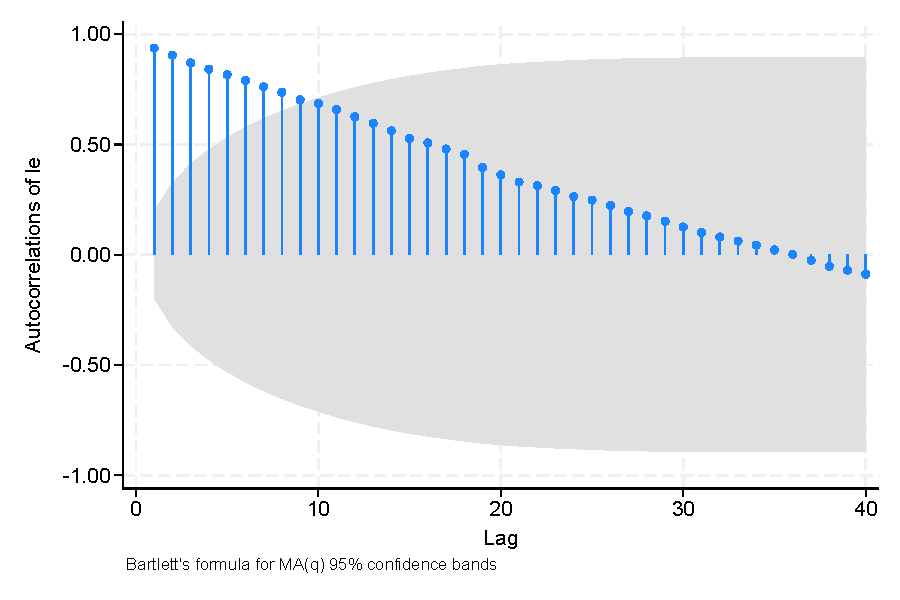
\includegraphics[width=0.45\textwidth]{image/acf.pdf} &
        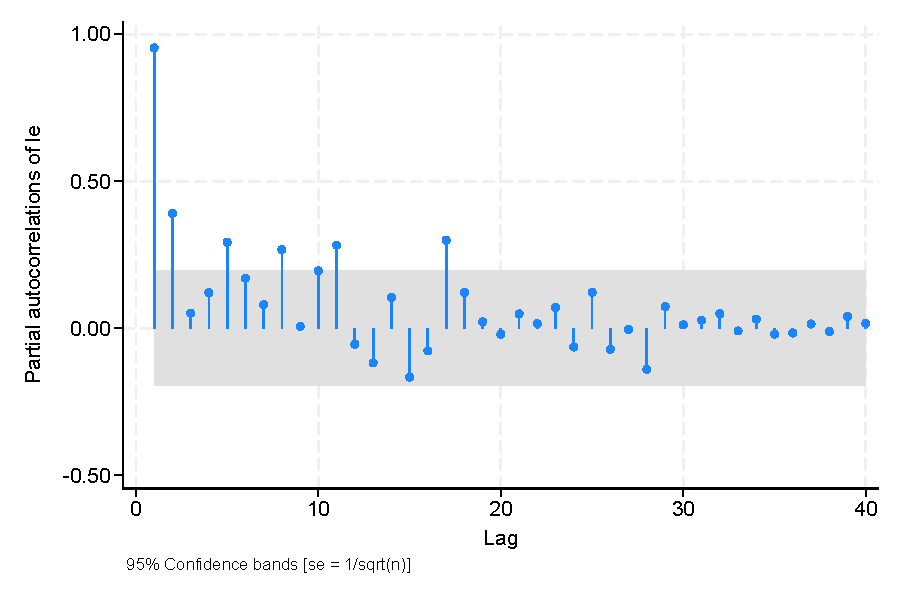
\includegraphics[width=0.45\textwidth]{image/pac.pdf}
    \end{tabular}}
    \caption{自相关图(左)和偏自相关图(右)}
    \label{fig:acf_pac}
\end{figure}

\begin{tcolorbox}[title=在 Stata 中应用多变量时间序列分析, colback=white, colframe=black, colbacktitle=white, coltitle=black,fonttitle=\bfseries]
\begin{lstlisting}[xleftmargin=2em, commentstyle=\color{black}]
webuse rates, clear
describe
summarize
tsset date, daily // 设定时间索引
// 此处应该检验单位根,限于篇幅省略
twoway (line dow date, lcolor(blue)) (line nasdaq date, lcolor(red))
display 12*(357/100)^0.25 // 参考陈强书书p418提及的内容,确定最大滞后阶数
varsoc dow nasdaq, maxlag(16) //根据AIC准则判断为8阶
var dow nasdaq, lags(1/8)
vargranger
irf create var_rates, set(rates_irf) replace
irf graph irf
irf graph fevd
*协整内容同上,var改成vec即可
vecrank dow nasdaq, max trend(none) // 约翰森协整检验
\end{lstlisting}
\vspace{-2em}
\begin{Verbatim}[commandchars=\\\{\},xleftmargin=2em]

. display 12*(357/100)^0.25 // 参考陈强书书p418提及的内容,确定最大滞后阶数
16.494847

. varsoc dow nasdaq, maxlag(16) //根据AIC准则判断为8阶

Lag-order selection criteria

   Sample: 09aug1960 thru 15jul1961                        Number of obs = 341
  +---------------------------------------------------------------------------+
  | Lag |    LL      LR      df    p     FPE       AIC      HQIC      SBIC    |
  |-----+---------------------------------------------------------------------|
  …………………………………………………………………………………………………………
  |   8 | -4064.79  23.451    4  0.000 9.5e+07*  24.0398*  24.1921   24.4219  |
  …………………………………………………………………………………………………………
  +---------------------------------------------------------------------------+
   * optimal lag
   Endogenous: dow nasdaq
    Exogenous: _cons

\end{Verbatim}
\end{tcolorbox}

\begin{tcolorbox}[title=在 Stata 中应用多变量时间序列分析, colback=white, colframe=black, colbacktitle=white, coltitle=black,fonttitle=\bfseries]

\begin{Verbatim}[commandchars=\\\{\},xleftmargin=2em]

    Vector autoregression

Sample: 01aug1960 thru 15jul1961                Number of obs     =        349
Log likelihood =  -4156.557                     AIC               =   24.01465
FPE            =   9.22e+07                     HQIC              =   24.16416
Det(Sigma_ml)  =   7.58e+07                     SBIC              =   24.39022

Equation           Parms      RMSE     R-sq      chi2     P>chi2
----------------------------------------------------------------
dow                  17     122.756   0.0721   27.09877   0.0404
nasdaq               17     76.8916   0.1067   41.70088   0.0004
----------------------------------------------------------------

------------------------------------------------------------------------------
             | Coefficient  Std. err.      z    P>|z|     [95% conf. interval]
-------------+----------------------------------------------------------------
………………………………………………………………………………………………………………
------------------------------------------------------------------------------

. vargranger

   Granger causality Wald tests
  +------------------------------------------------------------------+
  |          Equation           Excluded |   chi2     df Prob > chi2 |
  |--------------------------------------+---------------------------|
  |               dow             nasdaq |  17.905     8    0.022    |
  |               dow                ALL |  17.905     8    0.022    |
  |--------------------------------------+---------------------------|
  |            nasdaq                dow |  30.338     8    0.000    |
  |            nasdaq                ALL |  30.338     8    0.000    |
  +------------------------------------------------------------------+

\end{Verbatim}
\end{tcolorbox}

\begin{figure}[htbp]
    \centering
    \fbox{\begin{tabular}{cc}
        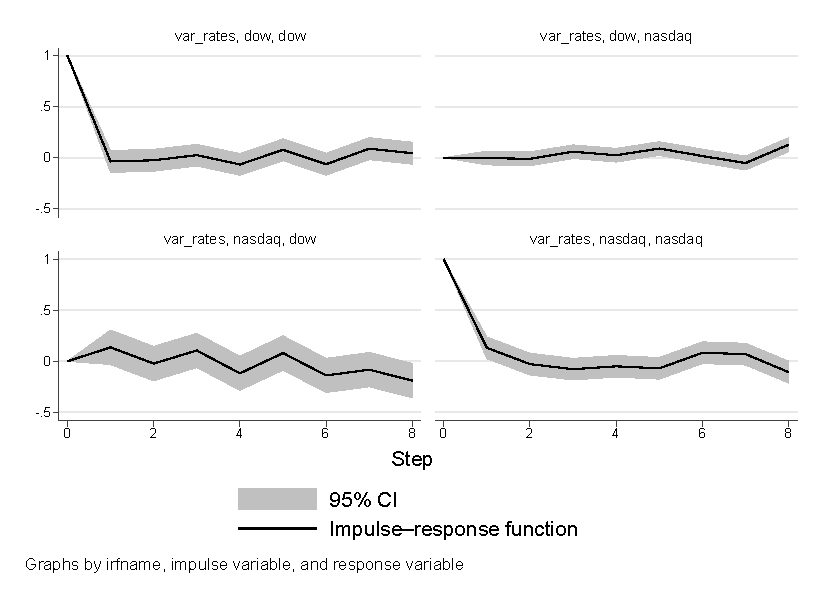
\includegraphics[width=0.45\textwidth]{image/Impulse_response.pdf} &
        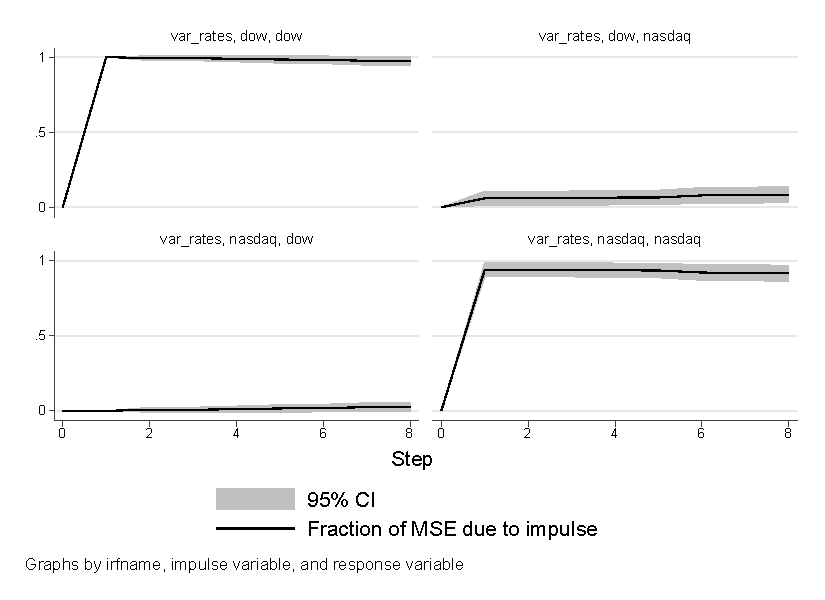
\includegraphics[width=0.45\textwidth]{image/FEVD.pdf}
    \end{tabular}}
    \caption{脉冲响应和残差分解}
    \label{fig:impulse response and residual decomposition}
\end{figure}

\begin{tcolorbox}[title=在 Stata 中应用多变量时间序列分析, colback=white, colframe=black, colbacktitle=white, coltitle=black,fonttitle=\bfseries]

\begin{Verbatim}[commandchars=\\\{\},xleftmargin=2em]

. vecrank dow nasdaq, max trend(none) // 约翰森协整检验

Johansen tests for cointegration
Trend: <none>                             Number of obs  = 355
Sample: 26jul1960 thru 15jul1961          Number of lags =   2
--------------------------------------------------------------
                                                      Critical
Maximum                                        Trace     value
   rank  Params           LL  Eigenvalue   statistic        5%
      0      4    -4397.1286           .    282.1329     12.53
      1      7    -4323.6287     0.33905    135.1329      3.84
      2      8    -4256.0622     0.31659
--------------------------------------------------------------
                                                      Critical
Maximum                        ------Eigenvalue-----     value
   rank  Params           LL                 Maximum        5%
      0      4    -4397.1286           .    147.0000     11.44
      1      7    -4323.6287     0.33905    135.1329      3.84
      2      8    -4256.0622     0.31659
--------------------------------------------------------------

\end{Verbatim}
\end{tcolorbox}

\subsection{空间计量经济学}
空间计量经济学处理的是截面或面板数据中,观测单元在地理空间上的相互依赖性。托布勒的地理学第一定律指出:“任何事物都与其他事物相关,但近处的事物比远处的事物更相关。”这种\textbf{空间依赖性(Spatial Dependence)}或\textbf{空间自相关(Spatial Autocorrelation)}违反了OLS观测独立的假定,会导致估计量有偏或无效。

\paragraph*{空间权重矩阵与空间自相关检验}
量化空间依赖性的关键工具是\textbf{空间权重矩阵(Spatial Weight Matrix, W)}。这是一个 $n \times n$ 的矩阵,其元素 $w_{ij}$ 反映了观测单元 $i$ 和 $j$ 之间的空间邻近程度。常见的设定包括:

\textbf{邻接矩阵}:如果 $i$ 和 $j$ 相邻,则 $w_{ij}=1$,否则为0。
\textbf{距离反比矩阵}:$w_{ij} = 1/d_{ij}$,其中 $d_{ij}$ 是两者间的距离。

通常对 $\mathbf{W}$ 进行行标准化,使得每行元素之和为1。

在进行空间回归之前,通常需要检验变量是否存在空间自相关。最常用的检验是\textbf{莫兰指数(Moran's I)},其值域通常在-1到1之间,正值表示空间集聚,负值表示空间分散,0表示空间随机分布。

\paragraph*{空间回归模型}
为处理空间依赖性,发展了多种空间回归模型:
\begin{enumerate}
    \item \textbf{空间滞后模型(Spatial Lag Model, SLM / SAR)}:假设因变量受到其邻近地区因变量的影响(空间溢出效应)。
    \begin{equation}
    \mathbf{Y} = \rho \mathbf{W}\mathbf{Y} + \mathbf{X}\boldsymbol{\beta} + \boldsymbol{\varepsilon}
    \end{equation}
    其中 $\rho$ 是空间自回归系数,衡量空间依赖的强度。

    \item \textbf{空间误差模型(Spatial Error Model, SEM)}:假设误差项存在空间相关性,即一个地区的冲击会影响到邻近地区。
    \begin{equation}
    \mathbf{Y} = \mathbf{X}\boldsymbol{\beta} + \mathbf{u}, \quad \text{其中 } \mathbf{u} = \lambda \mathbf{W}\mathbf{u} + \boldsymbol{\varepsilon}
    \end{equation}
    其中 $\lambda$ 是空间误差系数。

    \item \textbf{空间杜宾模型(Spatial Durbin Model, SDM)}:是更具一般性的模型,同时包含了因变量和自变量的空间滞后项。
    \begin{equation}
    \mathbf{Y} = \rho \mathbf{W}\mathbf{Y} + \mathbf{X}\boldsymbol{\beta} + \mathbf{W}\mathbf{X}\boldsymbol{\theta} + \boldsymbol{\varepsilon}
    \end{equation}
\end{enumerate}

在包含空间滞后项的模型(如SLM和SDM)中,系数 $\boldsymbol{\beta}$ 不能再解释为边际效应,因为存在反馈效应和溢出效应。需要分解为\textbf{直接效应(Direct Effect)}、\textbf{间接效应(Indirect Effect,即溢出效应)}和\textbf{总效应(Total Effect)}。


* 案例省略,可参见习明明《“傻瓜”计量经济学与Stata应用(第二版)》第十四到十七章。

\section{do算子与处置效应}

在前面的章节中,我们主要关注的是变量之间的关联性,即条件期望 $E(Y|X)$。然而,社会科学研究的最终目标往往是探寻因果关系——如果我们主动干预(intervene)变量 $X$,变量 $Y$ 会发生怎样的变化?这对应于一个不同的概念:$E(Y|\text{do}(X=x))$。

Judea Pearl 引入的 \textbf{do算子} 明确区分了“观察”(seeing)与“行动”(doing)。$E(Y|X=x)$ 描述的是,当我们观察到 $X$ 的值为 $x$ 时,对 $Y$ 的期望值是多少;而 $E(Y|\text{do}(X=x))$ 描述的是,当我们强制将 $X$ 设定为 $x$ 时(无论其自然状态如何),对 $Y$ 的期望值是多少。例如,观察到地面是湿的($X=1$)与下雨($Y=1$)高度相关,但如果我们人为地用水管把地面弄湿($\text{do}(X=1)$),并不会导致下雨。

do算子为我们思考因果问题提供了一个清晰的理论框架。在实证研究中,这种“干预”通常被称为\textbf{处置(Treatment)},而我们的目标就是识别和估计其产生的\textbf{处置效应(Treatment Effect)}。

\subsection{虚拟变量}
在估计处置效应时,最常见的变量类型之一就是\textbf{虚拟变量(Dummy Variable)},也称为指示变量(Indicator Variable)。它通常用于表示某个处置的有无、某个特征的存在与否,或某个体所属的类别。

\paragraph*{虚拟变量的定义与生成}
虚拟变量是一个取值为0或1的二元变量。例如,我们可以定义一个变量 $D_i$,如果个体 $i$ 接受了某项培训(处置组),则 $D_i=1$;如果未接受(控制组),则 $D_i=0$。

对于多分类变量,如个体的受教育程度(小学、中学、大学),我们可以创建一组虚拟变量来表示。假设有 $C$ 个类别,我们通常会生成 $C-1$ 个虚拟变量。

在 Stata 中,我们可以使用 \texttt{tabulate} 命令或因子变量表示法 \texttt{i.} 来快速生成虚拟变量。

\paragraph*{基准组与虚拟变量陷阱}
在上面的回归中,Stata自动将 \texttt{race} 类别中的“白人(white)”和 \texttt{industry} 类别中的“制造业(Manufacturing)”作为\textbf{基准组(Base Group)}或参照组。所有虚拟变量的系数都解释为相对于其基准组的差异。例如,\texttt{race} 类别中 \texttt{black} 的系数-1.54表示,在控制其他变量的情况下,黑人女性的平均工资比白人女性低1.54美元/小时。

如果我们试图将所有类别的虚拟变量(例如,白人、黑人、其他族裔三个虚拟变量)都放入包含截距项的模型中,就会导致\textbf{完全多重共线性},因为这三个虚拟变量之和恒等于1(即截距项)。这被称为\textbf{虚拟变量陷阱(Dummy Variable Trap)}。解决方法就是始终省略一个类别作为基准组。

\paragraph*{交互项与异质性效应}
虚拟变量的强大之处在于它可以与\textbf{其他}变量(无论是连续变量还是虚拟变量)构建\textbf{交互项(Interaction Term)},用以探究\textbf{异质性处置效应(Heterogeneous Treatment Effects)}。

例如,我们想知道教育回报率是否因种族而异。我们可以构建教育年限(\texttt{grade})和种族虚拟变量(\texttt{i.race})的交互项。

\begin{equation}
\text{wage} = \beta_0 + \beta_1 \text{black} + \beta_2 \text{grade} + \beta_3 (\text{black} \times \text{grade}) + \varepsilon
\end{equation}
在这个模型中:
\begin{itemize}
    \item 白人(基准组,$\text{black}=0$)的工资方程为:$E(\text{wage}|\text{black}=0) = \beta_0 + \beta_2 \text{grade}$。每增加一年教育,工资期望增加 $\beta_2$。
    \item 黑人($\text{black}=1$)的工资方程为:$E(\text{wage}|\text{black}=1) = (\beta_0 + \beta_1) + (\beta_2 + \beta_3) \text{grade}$。每增加一年教育,工资期望增加 $\beta_2 + \beta_3$。
\end{itemize}
交互项系数 $\beta_3$ 捕捉了教育回报率在黑人和白人之间的差异。如果 $\beta_3$ 显著不为零,则表明存在异质性效应。

\subsection{处置效应与偏误}
\paragraph*{反事实框架与处置效应}
为了严谨地定义因果效应,我们引入\textbf{潜在结果框架(Potential Outcomes Framework)},也称作Rubin因果模型。对每个个体 $i$,我们定义两个潜在结果:
\begin{itemize}
    \item $Y_i(1)$: 如果个体 $i$ 接受处置($D_i=1$),其可能的结果。
    \item $Y_i(0)$: 如果个体 $i$ 未接受处置($D_i=0$),其可能的结果。
\end{itemize}
个体 $i$ 的因果效应(处置效应)就是 $Y_i(1) - Y_i(0)$。然而,\textbf{因果推断的根本问题}在于,在同一时间点,我们只能观测到其中一个潜在结果。我们观测到的实际结果 $Y_i$ 可以表示为:
\begin{equation}
Y_i = D_i Y_i(1) + (1-D_i) Y_i(0)
\end{equation}
由于无法观测到个体的因果效应,我们转而关注总体的平均效应:
\begin{itemize}
    \item \textbf{平均处置效应 (Average Treatment Effect, ATE)}: $\text{ATE} = E[Y_i(1) - Y_i(0)]$
    \item \textbf{处置组的平均处置效应 (Average Treatment Effect on the Treated, ATT)}: $\text{ATT} = E[Y_i(1) - Y_i(0) | D_i=1]$
\end{itemize}

\paragraph*{选择性偏误}
一个很自然的想法是,直接比较处置组和控制组的平均结果差异来估计处置效应:
\begin{equation}
\Delta = E[Y_i | D_i=1] - E[Y_i | D_i=0]
\end{equation}
然而,这个简单的差异通常不等于ATE或ATT。我们可以将其分解:
\begin{align}
\Delta &= E[Y_i(1) | D_i=1] - E[Y_i(0) | D_i=0] \\
&= E[Y_i(1) | D_i=1] - E[Y_i(0) | D_i=1] + E[Y_i(0) | D_i=1] - E[Y_i(0) | D_i=0] \\
&= \text{ATT} + \underbrace{E[Y_i(0) | D_i=1] - E[Y_i(0) | D_i=0]}_{\text{选择性偏误 (Selection Bias)}}
\end{align}
\textbf{选择性偏误}来源于:即使处置组没有接受处置,他们的潜在结果 $Y_i(0)$ 也可能系统性地不同于控制组。例如,参加职业培训的人(处置组)可能本身就比不参加的人(控制组)更有上进心,因此即使不参加培训,他们的平均工资也可能更高。

随机对照实验(RCT)通过随机分配处置,确保了 $E[Y_i(0) | D_i=1] = E[Y_i(0) | D_i=0]$,从而消除了选择性偏误。但在无法进行实验的观测性研究中,我们就必须依赖各种\textbf{识别策略}来处理选择性偏误,这也是计量经济学中因果推断方法的核心任务。

\section{两种策略}

当随机实验不可行时,我们如何从观测数据中识别因果效应?核心在于找到一种方法来控制或消除选择性偏误。本节介绍两种基于“可观测特征”进行控制的策略:匹配法和回归法。这两种方法都依赖一个核心假设,即“条件独立性假设”(Conditional Independence Assumption, CIA),也称为“可忽略性”(Ignorability)或“基于可观测变量的选择”(Selection on Observables)。该假设认为,一旦我们控制了一组足够丰富的可观测变量 $\mathbf{X}$,处置的分配就可以被视为是随机的。

\begin{equation}
(Y_i(1), Y_i(0)) \perp D_i | \mathbf{X}_i
\end{equation}

\subsection{匹配法}
\paragraph*{基本思想}
匹配法的思想非常直观:为了估计处置对个体 $i$(假设其在处置组)的影响,我们在控制组中寻找一个或多个与个体 $i$ 在可观测特征 $\mathbf{X}$ 上“尽可能相似”的个体作为其反事实的代理。通过比较处置组个体与其匹配的控制组个体的平均结果差异,我们就可以得到一个消除了选择性偏误的处置效应估计。本质上,匹配是在观测数据中模拟一个“准实验”。

\paragraph*{倾向得分匹配}
当控制变量 $\mathbf{X}$ 的维度很高时,要找到特征完全相同的个体几乎是不可能的(这被称为\textbf{维度灾难 Curse of Dimensionality})。Rosenbaum 和 Rubin (1983) 证明,如果条件独立性假设成立,那么我们只需要在一个一维变量上进行匹配就足够了,这个变量就是\textbf{倾向得分(Propensity Score)}。
\begin{equation}
p(\mathbf{X}_i) = P(D_i=1|\mathbf{X}_i)
\end{equation}
倾向得分是在给定一系列可观测特征 $\mathbf{X}$ 的条件下,个体接受处置的概率。我们可以通过Logit或Probit模型来估计每个个体的倾向得分。

之后,我们就可以根据倾向得分进行匹配。常见的匹配算法包括:
\begin{itemize}
    \item \textbf{最近邻匹配(Nearest Neighbor Matching)}:为每个处置组个体,在控制组中寻找倾向得分最接近的一个或多个个体。
    \item \textbf{半径匹配(Radius/Caliper Matching)}:为每个处置组个体,匹配上所有倾向得分落在其一个特定半径(Caliper)范围内的控制组个体。
    \item \textbf{核匹配(Kernel Matching)}:为每个处置组个体,用其附近所有控制组个体的加权平均来构建反事实,权重由其与处置组个体的倾向得分距离决定。
\end{itemize}

\paragraph*{平衡性检验与共同支撑}
匹配的一个关键前提是\textbf{共同支撑(Common Support)},即对于任何倾向得分的取值,处置组和控制组中都存在个体。如果某些特征的个体只存在于处置组(或控制组),那我们就无法为他们找到合适的匹配。

匹配完成后,必须进行\textbf{平衡性检验(Balance Test)},检查匹配后处置组和控制组的 $\mathbf{X}$ 变量的分布是否变得相似(即均值无显著差异)。如果匹配后变量仍然不平衡,则说明倾向得分模型可能设定有误,需要重新设定模型再次匹配。

\subsection{回归法}
\paragraph*{回归模型的作用}
多元回归是另一种控制可观测变量 $\mathbf{X}$ 以估计处置效应的常用方法。其基本思想是,通过将 $\mathbf{X}$ 作为控制变量放入回归模型,我们可以“分离出”处置变量 $D$ 对结果变量 $Y$ 的净影响。
\begin{equation}
Y_i = \beta_0 + \tau D_i + \boldsymbol{\beta}' \mathbf{X}_i + \varepsilon_i
\end{equation}
在这个模型中,如果条件独立性假设成立,并且我们对函数形式(线性)的设定是正确的,那么系数 $\tau$ 就是对平均处置效应(ATE)的一个一致估计。它衡量的是,在保持 $\mathbf{X}$ 不变的情况下,接受处置($D=1$)与不接受处置($D=0$)的个体之间 $Y$ 的平均差异。

\paragraph*{交互项与异质性效应}
与虚拟变量部分讨论的类似,回归法可以非常方便地通过引入处置变量与协变量的交互项来检验和估计异质性处置效应。
\begin{equation}
Y_i = \beta_0 + \tau D_i + \beta_1 X_{1i} + \gamma (D_i \times X_{1i}) + \dots + \varepsilon_i
\end{equation}
此时,对于 $X_1$ 取值不同的个体,处置效应是不同的。处置效应变为 $\tau + \gamma X_{1i}$。

\paragraph*{与匹配法的比较}
匹配法和回归法都是基于“可观测变量的选择”这一核心假设,但它们实现控制的方式有所不同。
\begin{itemize}
    \item \textbf{函数形式}:回归法对 $Y$ 与 $D, \mathbf{X}$ 之间的关系施加了特定的函数形式(通常是线性的)。如果这种形式设定错误,估计就会产生偏误。匹配法是非参数的,不对函数形式做过多假设,因此更为稳健。
    \item \textbf{共同支撑}:匹配法强制要求在共同支撑域内进行比较,对于不在共同支撑域内的观测值会将其丢弃,这使得我们对估计结果的适用范围有更清醒的认识。回归法虽然在理论上也需要共同支撑,但它会利用函数形式进行外推,即使在数据稀疏的区域也会给出估计,这可能掩盖了共同支撑问题。
    \item \textbf{效率}:如果线性模型是正确的,回归法的估计通常比匹配法更有效率(即标准误更小)。
\end{itemize}

在实践中,这两种方法常常被结合使用,例如在匹配后的样本上再进行回归分析,以期获得既稳健又有效率的估计结果。这种方法被称为回归调整(Regression Adjustment)或双重稳健估计(Doubly Robust Estimation)。